\documentclass[11pt,twoside,a4paper,openright]{report}
%%%%%%%%%%%%%%%%%%%%%%%%%%%%%%%%%%%%%%%%%%%%%%%%
% Language, Encoding and Fonts
% http://en.wikibooks.org/wiki/LaTeX/Internationalization
%%%%%%%%%%%%%%%%%%%%%%%%%%%%%%%%%%%%%%%%%%%%%%%%
% Select encoding of your inputs. Depends on
% your operating system and its default input
% encoding. Typically, you should use
%   Linux  : utf8 (most modern Linux distributions)
%            latin1 
%   Windows: ansinew
%            latin1 (works in most cases)
%   Mac    : applemac
% Notice that you can manually change the input
% encoding of your files by selecting "save as"
% an select the desired input encoding. 
\usepackage[utf8]{inputenc}
% Make latex understand and use the typographic
% rules of the language used in the document.
\usepackage[danish,english]{babel}
% Use the palatino font
\frenchspacing
\usepackage[sc]{mathpazo}
\linespread{1.05}         % Palatino needs more leading (space between lines)
% Choose the font encoding
\usepackage[T1]{fontenc}
%Symbol dictionary package(used for tick symbol)
\usepackage{bbding}

%%%%%%%%%%%%%%%%%%%%%%%%%%%%%%%%%%%%%%%%%%%%%%%%
% Graphics and Tables
% http://en.wikibooks.org/wiki/LaTeX/Importing_Graphics
% http://en.wikibooks.org/wiki/LaTeX/Tables
% http://en.wikibooks.org/wiki/LaTeX/Colors
%%%%%%%%%%%%%%%%%%%%%%%%%%%%%%%%%%%%%%%%%%%%%%%%
% load a colour package
\usepackage{xcolor}
\definecolor{aaublue}{RGB}{33,26,82}% dark blue
% The standard graphics inclusion package
\usepackage{graphicx}
% Set up how figure and table captions are displayed
\usepackage{subcaption}
\usepackage{caption}
\captionsetup{%
  font=footnotesize,% set font size to footnotesize
  labelfont=bf % bold label (e.g., Figure 3.2) font
}
% Make the standard latex tables look so much better
\usepackage{array,booktabs,tabularx,multirow}
% Enable the use of frames around, e.g., theorems
% The framed package is used in the example environment
\usepackage{framed}

% Adds support for full page background picture
\usepackage[contents={},color=gray]{background}
%\usepackage[contents=draft,color=gray]{background}

%%%%%%%%%%%%%%%%%%%%%%%%%%%%%%%%%%%%%%%%%%%%%%%%
% Mathematics
% http://en.wikibooks.org/wiki/LaTeX/Mathematics
%%%%%%%%%%%%%%%%%%%%%%%%%%%%%%%%%%%%%%%%%%%%%%%%
% Defines new environments such as equation,
% align and split 
\usepackage{mathtools}
% Adds new math symbols
\usepackage{amssymb}
% Use theorems in your document
% The ntheorem package is also used for the example environment
% When using thmmarks, amsmath must be an option as well. Otherwise \eqref doesn't work anymore.
\usepackage[framed,amsmath,thmmarks]{ntheorem}

%%%%%%%%%%%%%%%%%%%%%%%%%%%%%%%%%%%%%%%%%%%%%%%%
% Page Layout
% http://en.wikibooks.org/wiki/LaTeX/Page_Layout
%%%%%%%%%%%%%%%%%%%%%%%%%%%%%%%%%%%%%%%%%%%%%%%%
% Change margins, papersize, etc of the document
\usepackage[
  inner=28mm,% left margin on an odd page
  outer=41mm,% right margin on an odd page
  headheight=13.6pt,
  bottom=39mm
  ]{geometry}
% Modify how \chapter, \section, etc. look
% The titlesec package is very configureable
\usepackage{titlesec}
\titleformat{\chapter}[display]{\normalfont\huge\bfseries}{\chaptertitlename\ \thechapter}{20pt}{\Huge}
\titleformat*{\section}{\normalfont\Large\bfseries}
\titleformat*{\subsection}{\normalfont\large\bfseries}
\titleformat*{\subsubsection}{\normalfont\normalsize\bfseries}
%\titleformat*{\paragraph}{\normalfont\normalsize\bfseries}
%\titleformat*{\subparagraph}{\normalfont\normalsize\bfseries}

% Clear empty pages between chapters
\let\origdoublepage\cleardoublepage
\newcommand{\clearemptydoublepage}{%
  \clearpage
  {\pagestyle{empty}\origdoublepage}%
}
\let\cleardoublepage\clearemptydoublepage

% Change the headers and footers
\usepackage{fancyhdr}
\pagestyle{fancy}
\fancyhf{} %delete everything
\renewcommand{\headrulewidth}{0pt} %remove the horizontal line in the header
\fancyhead[RE]{\small\nouppercase\leftmark} %even page - chapter title
\fancyhead[LO]{\small\nouppercase\rightmark} %uneven page - section title
\fancyhead[LE,RO]{\thepage \hspace{1pt} of \pageref{LastPage}} %page number on all pages
% Do not stretch the content of a page. Instead,
% insert white space at the bottom of the page
\raggedbottom
% Enable arithmetics with length. Useful when
% typesetting the layout.
\usepackage{calc}

%%%%%%%%%%%%%%%%%%%%%%%%%%%%%%%%%%%%%%%%%%%%%%%%
% Bibliography
% http://en.wikibooks.org/wiki/LaTeX/Bibliography_Management
%%%%%%%%%%%%%%%%%%%%%%%%%%%%%%%%%%%%%%%%%%%%%%%%
\usepackage[backend=biber,
  bibencoding=utf8,
  maxbibnames=20,
  style=numeric-comp,
  sorting=none
  ]{biblatex}
\addbibresource{bib/mybib.bib}
\usepackage{microtype} %Prevent overfull issues in bibliography

%%%%%%%%%%%%%%%%%%%%%%%%%%%%%%%%%%%%%%%%%%%%%%%%
% Misc
%%%%%%%%%%%%%%%%%%%%%%%%%%%%%%%%%%%%%%%%%%%%%%%%
% Add bibliography and index to the table of
% contents
\usepackage[nottoc]{tocbibind}
% Add the command \pageref{LastPage} which refers to the
% page number of the last page
\usepackage{lastpage}
% Add todo notes in the margin of the document
\usepackage[
%  disable, %turn off todonotes
  colorinlistoftodos, %enable a coloured square in the list of todos
  textwidth=\marginparwidth, %set the width of the todonotes
  textsize=scriptsize, %size of the text in the todonotes
  ]{todonotes}

%%%%%%%%%%%%%%%%%%%%%%%%%%%%%%%%%%%%%%%%%%%%%%%%
% Code listings and pseudocode
\usepackage[newfloat, outputdir=out]{minted}
\setminted[python]{frame=topline, framesep=6pt, style=colorful, fontsize=\footnotesize, linenos, breaklines, autogobble} %Change language later
\setminted[text]{frame=topline, framesep=6pt, fontsize=\footnotesize, linenos, breaklines, autogobble}
\usepackage{clrscode3e}
\DeclareFloatingEnvironment[name=Algorithm, placement=htp!]{algorithm} %Create Algorithm float

%%%%%%%%%%%%%%%%%%%%%%%%%%%%%%%%%%%%%%%%%%%%%%%%
% Hyperlinks
% http://en.wikibooks.org/wiki/LaTeX/Hyperlinks
%%%%%%%%%%%%%%%%%%%%%%%%%%%%%%%%%%%%%%%%%%%%%%%%
% Enable hyperlinks and insert info into the pdf
% file. Hypperref should be loaded as one of the 
% last packages
\usepackage[hidelinks]{hyperref}
\hypersetup{%
	plainpages=false,%
	pdfauthor={Author(s)},%
	pdftitle={Title},%
	pdfsubject={Subject},%
	bookmarksnumbered=true,%
	colorlinks=false,%
	citecolor=black,%
	filecolor=black,%
	linkcolor=black,% you should probably change this to black before printing
	urlcolor=black,%
	pdfstartview=FitH%
}

\usepackage[acronym]{glossaries} %Glossaries/acronyms
\usepackage[autostyle, threshold=0]{csquotes} %better quotes

% see, e.g., http://en.wikibooks.org/wiki/LaTeX/Formatting#Hyphenation
% for more information on word hyphenation
\hyphenation{ex-am-ple hy-phen-a-tion short}
\hyphenation{long la-tex}

\newcommand{\aautitlepage}[3]{%
  {
    %set up various length
    \ifx\titlepageleftcolumnwidth\undefined
      \newlength{\titlepageleftcolumnwidth}
      \newlength{\titlepagerightcolumnwidth}
    \fi
    \setlength{\titlepageleftcolumnwidth}{0.5\textwidth-\tabcolsep}
    \setlength{\titlepagerightcolumnwidth}{\textwidth-2\tabcolsep-\titlepageleftcolumnwidth}
    %create title page
    \thispagestyle{empty}
    \noindent%
    \begin{tabular}{@{}ll@{}}
      \parbox{\titlepageleftcolumnwidth}{
        \iflanguage{danish}{%
          
\includegraphics[width=\titlepageleftcolumnwidth]{figures/AAUgraphics/aau_logo_da}
        }{%
          
\includegraphics[width=\titlepageleftcolumnwidth]{figures/AAUgraphics/aau_logo_en}
        }
      } &
      \parbox{\titlepagerightcolumnwidth}{\raggedleft\sf\small
        #2
      }\bigskip\\
       #1 &
      \parbox[t]{\titlepagerightcolumnwidth}{%
      \textbf{Abstract:}\par
        \fbox{\parbox{\titlepagerightcolumnwidth-2\fboxsep-2\fboxrule}{%
          #3
        }}
      }\\
    \end{tabular}
    \vfill
    \iflanguage{danish}{%
      \noindent{\footnotesize\emph{Rapportens indhold er frit tilgængeligt, men offentliggørelse (med kildeangivelse) må kun ske efter aftale med forfatterne.}}
    }{%
      \noindent{\footnotesize\emph{The content of this report is freely available, but publication (with reference) may only be pursued due to agreement with the author.}}
    }
    \clearpage
  }
}

%Create english project info
\newcommand{\englishprojectinfo}[8]{%
  \parbox[t]{\titlepageleftcolumnwidth}{
    \textbf{Title:}\\ #1\bigskip\par
    \textbf{Theme:}\\ #2\bigskip\par
    \textbf{Project Period:}\\ #3\bigskip\par
    \textbf{Project Group:}\\ #4\bigskip\par
    \textbf{Participant(s):}\\ #5\bigskip\par
    \textbf{Supervisor(s):}\\ #6\bigskip\par
    \textbf{Copies:} #7\bigskip\par
    \textbf{Page Numbers:} \pageref{LastPage}\bigskip\par
    \textbf{Date of Completion:}\\ #8
  }
}

%Create danish project info
\newcommand{\danishprojectinfo}[8]{%
  \parbox[t]{\titlepageleftcolumnwidth}{
    \textbf{Titel:}\\ #1\bigskip\par
    \textbf{Tema:}\\ #2\bigskip\par
    \textbf{Projektperiode:}\\ #3\bigskip\par
    \textbf{Projektgruppe:}\\ #4\bigskip\par
    \textbf{Deltager(e):}\\ #5\bigskip\par
    \textbf{Vejleder(e):}\\ #6\bigskip\par
    \textbf{Oplagstal:} #7\bigskip\par
    \textbf{Sidetal:} \pageref{LastPage}\bigskip\par
    \textbf{Afleveringsdato:}\\ #8
  }
}

%%%%%%%%%%%%%%%%%%%%%%%%%%%%%%%%%%%%%%%%%%%%%%%%
% An example environment
%%%%%%%%%%%%%%%%%%%%%%%%%%%%%%%%%%%%%%%%%%%%%%%%
\theoremheaderfont{\normalfont\bfseries}
\theorembodyfont{\normalfont}
\theoremstyle{break}
\def\theoremframecommand{{\color{gray!50}\vrule width 5pt \hspace{5pt}}}
\newshadedtheorem{exa}{Example}[chapter]
\newenvironment{example}[1]{%
		\begin{exa}[#1]
}{%
		\end{exa}
}

%%%%%%%%%%%%%%%%%%%%%%%%%%%%%%%%%%%%%%%%%%%%%%%%
% Specialized todo macros
%%%%%%%%%%%%%%%%%%%%%%%%%%%%%%%%%%%%%%%%%%%%%%%%
\newcommand{\supervisor}[2][]{\todo[color=green!50,#1]{#2}}
\newcommand{\question}[2][]{\todo[color=cyan!30,#1]{#2}}
\newcommand{\urgent}[2][]{\todo[color=red!50,#1]{#2}}
\newcommand{\feedback}[2][]{\todo[color=teal!70,#1]{#2}}

%import glossaries
\makeglossaries
\loadglsentries{setup/acronyms.tex}

\begin{document}
%frontmatter
\pagestyle{empty} %disable headers and footers
\pagenumbering{roman} %use roman page numbering in the frontmatter
\pdfbookmark[0]{Front page}{label:frontpage}%
\begin{titlepage}
\vspace*{\fill}
    \backgroundsetup{
    scale=1.1,
    angle=0,
    opacity=1.0,  %% adjust
    contents={
\includegraphics[width=\paperwidth,height=\paperheight]{figures/AAUgraphics/aau_waves}}
    }
  \addtolength{\hoffset}{0.5\evensidemargin-0.5\oddsidemargin} %set equal margins on the frontpage - remove this line if you want default margins
  \noindent%
  {\color{white}\fboxsep0pt\colorbox{aaublue}{\begin{tabular}{@{}p{\textwidth}@{}}
    \begin{center}
    \Huge{\textbf{
      Some Title% insert your title here
    }}
    \end{center}
    \begin{center}
      \Large{
        Some subtitle% insert your subtitle here
      }
    \end{center}
    \vspace{0.2cm}
   \begin{center}
    {\Large
      Daniel Runge Petersen, Nutsy Superman% insert names separated by comma
    }\\
    \vspace{0.2cm}
    {\large
      Computer Science, xXx% insert name of study, group number, year-month
    }
   \end{center}
   \vspace{0.2cm}
   \begin{center}
    {\Large
      Semester Project
      %Bachelor Project
      %Master's Project
    }
   \end{center}
  \end{tabular}}}
  \vfill
  \begin{center}
    
\includegraphics[width=0.2\paperwidth]{figures/AAUgraphics/aau_logo_circle_en}% comment this line in for English version
    %
\includegraphics[width=0.2\paperwidth]{figures/AAUgraphics/aau_logo_circle_da} %comment this line in for Danish version
  \end{center}
\end{titlepage}
\clearpage

\thispagestyle{empty}
{\small
\strut\vfill % push the content to the bottom of the page
\noindent Copyright \copyright{} Aalborg University 2021\par
\vspace{0.2cm}
\noindent Composed and typeset by the authors using the \LaTeX\ Document Preparation System, based on the AAU report template by~\citeauthor{Drunge}~\cite{Drunge}.
}
\clearpage


\pdfbookmark[0]{English title page}{label:titlepage_en}
\aautitlepage{%
  \englishprojectinfo{
    Project Title %title
  }{%
    Scientific Theme %theme
  }{%
    Fall Semester 2022 %project period
  }{%
    xXx % project group
  }{%
    %list of group members
    Daniel Runge Petersen\\
    Nutsy Superman
  }{%
    %list of supervisors
    Supervisor 1\\
    Supervisor 2
  }{%
    1 % number of printed copies
  }{%
    \today % date of completion
  }%
}{%department and address
  \textbf{Electronics and IT}\\
  Aalborg University\\
  \href{http://www.aau.dk}{http://www.aau.dk}
}{% the abstract
  This is the abstract.
}

\cleardoublepage
{\selectlanguage{danish}
\pdfbookmark[0]{Danish title page}{label:titlepage_da}
\aautitlepage{%
  \danishprojectinfo{
    Rapportens titel %title
  }{%
    Semestertema %theme
  }{%
    Efterårssemestret 2010 %project period
  }{%
    XXX % project group
  }{%
    %list of group members
    Forfatter 1\\ 
    Forfatter 2\\
    Forfatter 3
  }{%
    %list of supervisors
    Vejleder 1\\
    Vejleder 2
  }{%
    1 % number of printed copies
  }{%
    \today % date of completion
  }%
}{%department and address
  \textbf{Elektronik og IT}\\
  Aalborg Universitet\\
  \href{http://www.aau.dk}{http://www.aau.dk}
}{% the abstract
  Her er resuméet
}}
\cleardoublepage

\pdfbookmark[0]{Contents}{label:contents}
\pagestyle{fancy} %enable headers and footers again
\setcounter{tocdepth}{1} %determine depth of table of contents. 0 - 4
\tableofcontents

\chapter*{Preface\markboth{Preface}{Preface}}\label{ch:preface}
\addcontentsline{toc}{chapter}{Preface}
This report is written by group cs-22-dat-5-05, 5th semester at AAU. The theme of the report is "Theoretical data analysis and modeling", and is completed at the end of the fall semester of 2022.

The report has been completed with help from our supervisor, Alexander Leguizamon Robayo.

\vspace{\baselineskip}\hfill Aalborg University, \today
\vfill\noindent
\begin{center}
    \begin{minipage}[b]{0.45\textwidth}
        \centering
        \rule{\textwidth}{0.5pt}
        Daniel Runge Petersen\\
        {\footnotesize <username@student.aau.dk>}
    \end{minipage}
    \hfill
    \begin{minipage}[b]{0.45\textwidth}
        \centering
        \rule{\textwidth}{0.5pt}\\
        Gustav Svante Graversen\\
        {\footnotesize <username@student.aau.dk>}
    \end{minipage}
\end{center}
\vspace{2\baselineskip}
\begin{center}
    \begin{minipage}[b]{0.45\textwidth}
        \centering
        \rule{\textwidth}{0.5pt}
        Lars Emanuel Hansen\\
        {\footnotesize <usernamestudent.aau.dk>}
    \end{minipage}
    \hfill
    \begin{minipage}[b]{0.45\textwidth}
        \centering
        \rule{\textwidth}{0.5pt}\\
        Raymond Kacso\\
        {\footnotesize <username@student.aau.dk>}
    \end{minipage}
\end{center}
\vspace{2\baselineskip}
\begin{center}
    \begin{minipage}[b]{0.45\textwidth}
        \centering
        \rule{\textwidth}{0.5pt}
        Sebastian Aaholm\\
        {\footnotesize <username@student.aau.dk>}
    \end{minipage}
\end{center}
\vspace{2\baselineskip}


\cleardoublepage

%mainmatter
\pagenumbering{arabic} %use arabic page numbering in the mainmatter

\chapter{Introduction}\label{cha:introduction}
\todo[inline]{Chapter should probably contain: The initial problem (If we have one), motivation, and the scope or background of the project or theme. Report outline at the end.}
\noindent
In this project we will study some common methods of dimensionality reduction using the MNIST dataset for digit recognition.

\paragraph{Keywords:} dimensionality reduction, linear methods, nonlinear methods, MNIST, Computer Vision (CV), Machine Learning, machine intelligence (artificial intelligence).

Use sources \cite{IBM-machine-intelligence} and \cite{IBM-computer-vision} for superficial overview and explanations of umbrella terms.


Dimensionality reduction is a important topic in the field of \gls{ml}. The goal of dimensionality reduction is to reduce the number of features in a dataset while retaining as much relevant information as possible. This can be useful for improving the performance of \gls{ml} algorithms, as well as for visualizing and understanding the structure of a dataset ~\cite{dimensionality-reduction-cheng}. In this report, we focus on the comparison of two different dimensionality reduction techniques: linear and nonlinear methods.

Linear methods for dimensionality reduction, such as \gls{pca}, are widely used and have been well studied. These methods are computationally efficient and often perform well on a variety of tasks ~\cite{james-statistical-learning1}. However, nonlinear methods, such as \gls{kpca} are also relevant due to  their ability to capture more complex structures in a dataset ~\cite{dimensionality-reduction-cheng}. In this report, we aim to compare the relative effectiveness of these two types of dimensionality reduction methods.

We evaluate the performance of linear and nonlinear dimensionality reduction techniques on the \gls{mnist} dataset, a popular benchmark for image classification and recognition tasks. We use a \gls{svm} model to classify the images in the reduced datasets and compare the performance of the model under different settings. Our results provide valuable insights into the relative effectiveness of linear and nonlinear methods for dimensionality reduction in the context of \gls{cv}.

Overall, this report is of interest to researchers and practitioners in the field of \gls{ml} and \gls{cv}. Our findings have implications for the use of dimensionality reduction techniques in image classification and recognition tasks, and can inform future research in this area. By comparing linear and nonlinear methods, we aim to shed light on the relative strengths and limitations of these techniques and provide guidance for their practical use.





Notes to self: Humans vs computers in \gls{nn}. Why are humans good with little training, and computers only accceptable with much more training? Consider perhaps domains (recongnizing epsilon vs. recognizing a 3)

% Might be relevant to us: MNIST and fashion-MNIST (https://github.com/zalandoresearch/fashion-mnist).

\subsection*{On theory driven projects}
\blockcquote{Projectmodule}{The overall purpose of the project module is for the student to acquire the ability to analyze and evaluate the application of methods and techniques within database systems and / or machine intelligence to solve a specific problem. \textbf{This includes analyzes of the formal properties of the techniques and an assessment of these properties in relation to any requirements for the solution to the specific problem}. [...]

In this project module, the project work is primarily driven by theoretical and analytical considerations about the methods and techniques used. For a specific problem area, a project could, for example, be based on specific performance requirements for the developed software solution, and the project work can thus be guided by the solution's algorithmic time / space complexity as well as formal analyzes and considerations of its theoretical properties and performance guarantees.}

\section{Motivation}\label{sec:motivation}
High-dimensional data (i.e.\ data that requires more than three dimensions to be represented) can often be difficult to work with. Not only is it difficult to interpret and visualize but also can require a high use of computational resources. For these (and many more) reasons, it is important to study dimensionality reduction methods. These methods are usually used in exploratory data analysis and for visualization purposes.

The most usual methods of dimensionality reduction are \textbf{linear methods}. These methods might assume that the features in the original data are independent and they can produce reduced data by a linear combination of the original data. These assumptions might not apply to all datasets. In fact, there are cases in which linear methods do not capture important features of a dataset. For these cases one can use \textbf{nonlinear methods}. These methods can be used for more general cases while preserving important information from data.
\section{Report outline}\label{sec:report-outline}
The report is structured as follows:

\begin{itemize}
  \item \textbf{Introduction} - This chapter
  \item \textbf{Problem Analysis} - Chapter \ref{cha:problem-analysis}
  \item \textbf{Theory} - Chapter \ref{cha:theory}
  \item \textbf{Methodology} - Chapter \ref{cha:methodology}
  \item \textbf{Results} - Chapter \ref{cha:results}
  \item \textbf{Discussion} - Chapter \ref{cha:discussion}
  \item \textbf{Conclusion} - Chapter \ref{cha:conclusion}
\end{itemize}

The introduction describes the initial problem and the motivation for the project.

The Problem Analysis chapter dives into the initial problem and leads to a final problem statement.

The Methodology chapter describes the methods and theory used to explore the problem statement. It also describes the data used and how it was collected/created.

The Results chapter is an evaluation of the results of the project.

The Discussion chapter is a discussion of the results and the project as a whole.

The Conclusion chapter provides a summary of the project and the results. It also provides perspective and reflection on the project and the process.

\chapter{Problem analysis}\label{cha:problem-analysis}
This chapter describes the motivation for the project, culminating in a problem statement.

% \begin{itemize}
%     \item Why Machine learning + Generalized pipeline overview?
%     \item Why Feature Engineering: Dimensionality reduction
%           \begin{itemize}
%               \item Extraction
%               \item Visualization
%               \item Learning/debugging
%           \end{itemize}
%     \item Linear versus nonlinear methods
%     \item Problem statement
% \end{itemize}

\gls{ml} is a field of study within \gls{ai} concerned with learning from data, where learning means that data is analyzed and something is gathered from it. This could be methods to solve a puzzle, or patterns to recognize a number from an image. \gls{ml} is a complex and growing field used in many areas. One of the reasons for the increasing interest in \gls{ml} is the increasing amount of available data. The amount of data collected in the world is increasing at an incredible rate, which is expected to continue in the future~\cite{data-never-sleeps}. Because \gls{ml} models are trained on data, the more data available, the better the models can be~\cite{Unreasonable-effectiveness-of-data-Norvig}.

\gls{ml} can very generally be described as the discipline of teaching computers how to complete tasks, where no perfect algorithm is possible. This also covers when there are many possible good ways to achieve something, for this all the accepteble methods are then labeled as acceptable ways to succeed. These answers are then used to "train" the computer to improve on some basic algorithm\cite{alpaydin2020introduction}.

Inside a field as complex as \gls{ml} there exist many challenges, one such challenge is working with high-dimensional data. This is due to the inherent properties of many dimensions which makes it difficult to interpret and also computationally expensive. Higher dimensions are also associated with the so-called "curse of dimensionality". This term was coined by Richard E. Bellman in a paper about dynamic programming\cite{bellmanrand}. This term is used interchangeably with the terms 'peaking phenomenon' and 'Hughes phenomenon' \cite{koutroumbas2008pattern} \cite{hughes1968mean}. McLachlan states that:

“For training samples of a finite size, the performance of a given discriminant
rule in a frequentist framework does not keep on improving as the number p
of feature variables is increased. Rather, its overall unconditional error rate
will stop decreasing and start to increase as pis increased beyond a certain
threshold.” \cite{mclachlan2004s100}.

These difficulties associated with data in many dimensions, make the study of dimensionality reduction highly relevant. The goal of dimensionality reduction is to reduce the number of dimensions in a dataset, while retaining as much information as possible. This is done by extracting features from the data, which are then used to train a model. The extracted features are then used to make predictions on new data. This is a very general overview of the process of dimensionality reduction, and will be discussed in more detail in the next chapter.
it will be explained what it is and some of its uses in the following paragraphs.

% The most usual methods of dimensionality reduction are linear methods. These
% methods might assume that the features in the original data are independent and
% they can produce reduced data by a linear combination of the original data. These
% assumptions might not apply to all datasets. In fact, there are cases in which linear
% methods do not capture important features of a dataset. For these cases one can
% use nonlinear methods/ These methods can be used for more general cases while
% preserving important information from data


% However the complexity of \gls{ml} is also high. There are many different \gls{ml} models, each with different strengths and weaknesses. The choice of \gls{ml} model is therefore more often than not dependent on the data and the problem being solved. This means that choosing the right \gls{ml} model is a difficult task, which is further complicated by the fact that there is no single metric for evaluating the performance of a \gls{ml} model. The performance of a \gls{ml} model is often evaluated using multiple metrics, which makes it difficult to compare the performance of different models against each other.

% It may be necessary to try out different \gls{ml} models to find the best one for a certain problem, which is a time-consuming process.

% \section{Feature engineering}\label{sec:feature-engineering}
% % kort forklaring af FE, hvad er det 
% In machine learning \gls{fe} is used to transform the raw data into some type of data that is more suitable for the \gls{ml} model. A feature must derive from what type of data is given, and it is also tied to which model is being used. Some features are more appropriate for some types of models and vice versa. Feature engineering is the process of formulating the best fitted features given the task in hand, with the data and the chosen model~\cite{Feature-engineering-zheng}.

% There are many techniques for \gls{fe}, some examples on how to do \gls{fe} are: Imputation, handling outliers, scaling, dimensionality reduction. Imputation is the process of filling in missing values in the data. Most imputation is done by finding it by matrixes, by looking at other values in the dataset, a popular approach is k-nearest neighbors to find the missing values~\cite{imputation-for-tables-Biessmann}. Outliers are values that are far away from the rest of the data, and they can be a problem for some models, for both accuracy and inaccurate classification. It it therefore a good idea to eliminate the outliers, this is also a standard practice in most machine learning problems. There are many ways to handle outliers, one way is to remove them, another way is to replace them with the median or the mean of the data~\cite{outlier-perez}. 

% Scaling, also called feature normalization, is the process of transforming the data into a form that is more suitable for the \gls{ml} model. This is done by changing the range of the data, for example, if the data is in the range of 0-100, it can be scaled to be in the range of 0-1. This is done to make the data more suitable for the model, and to make it easier to compare the data. Scaling is also a standard practice in most machine learning problems. There are many ways to scale the data, one way is to use the min-max scaler, another way is to use variance scaling~\cite{Feature-engineering-zheng}.

% One of the goals of the dimensionality reduction methods is to counter the curse of dimensionality.
% According to Lee~\cite{nonlinear-dim-red-chapter-one}, the curse of dimensionality refers to "the number of data samples requried to estimate a function of several variables to a given accuracy on a given domain grows exponentially with the number of dimensions"~\cite{nonlinear-dim-red-chapter-one}. This means that machine learning models' performance might get affected by the huge amount of data that needs to be given.

% That is not optimal if we know that we can reduce the amount of data without losing too much information. On the contrary, the performance can perhaps be improved, partly because the size of the data gets reduced, and partly because the essence of the data is preserved. Dimensionality reduction will be further discussed in chapter~\ref{cha:theory}.

\section{dimensionality reduction}\label{sec:dimensionality-reduction-problem}

Dimmensionality is achieved by reducing the number of features(dimensions) in a dataset. This for example can help to visualize the data, or within a large dataset, describe which data weighs heavier on the expected output of the \gls{ml} model. Therefore, when reducing features in a dataset it is important to find the features that are more relevant to the output of the model~\cite{Feature-engineering-zheng}. There are many ways to reduce the dimensionality of a dataset, the different types of dimensionality reduction will be further discussed in Chapter~\ref{cha:theory}.

There are many dimensionality reduction methods and is still being researched today~\cite{dimensionality-reduction-cheng}. For example, these methods can improve heuristic models for explaining the data from surveys better through better visualizations, which is a good metric for evaluating surveys, since it improves understanding~\cite{dimensionality-reduction-cheng}.

When discussing which dimensionality reduction method is best it is important to consider what is most important for the method, in~\cite{dimensionality-reduction-maitra} they investigate which method is best for computational graph theory, using known methods in \gls{pca} and \gls{lda} for finding the best model.

In~\cite{dimensionality-reduction-reddy} they compare \gls{pca} and \gls{lda} on which is best on the Cardiotocography dataset with different \gls{ml} methods, and find that \gls{pca} outperforms \gls{lda}. In~\cite{dimensionality-reduction-comparative-review} they compare \gls{pca} with different nonlinear dimensionality reduction methods with artificial and natural datasets. They find that nonlinear methods perform well on artificial datasets, but not on natural datasets, as \gls{pca} does.

There are many methods and uses, so we will categorize dimensionality reduction into two general categories in the following section. Linear and nonlinear dimensionality reduction.

% Forklar hvorfor vi har valgt at fokusere på dimensionalitets reduction 


% @book{Feature-engineering-zheng,
% author = {Zheng, Alice and Casari, Amanda},
% title = {Feature Engineering for Machine Learning: Principles and Techniques for Data Scientists},
% year = {2018},
% isbn = {1491953241},
% }

% @article{imputation-for-tables-Biessmann,
%   author  = {Felix Biessmann and Tammo Rukat and Phillipp Schmidt and Prathik Naidu and Sebastian Schelter and Andrey Taptunov and Dustin Lange and David Salinas},
%   title   = {DataWig: Missing Value Imputation for Tables},
%   year    = {2019},
%   url     = {http://jmlr.org/papers/v20/18-753.html}
% }

% @article{outlier-perez,
% author = {Perez, Husein and Tah, Joseph H. M.},
% title = {Improving the Accuracy of Convolutional Neural Networks by Identifying and Removing Outlier Images in Datasets Using t-SNE},
% year = {2020},
% url = {https://www.mdpi.com/2227-7390/8/5/662},
% ISSN = {2227-7390},
% DOI = {10.3390/math8050662}
% }

%@book{nonlinear-dim-red-chapter-one,
% author={Lee, John A. and Verleysen, Michel},
% title={High-Dimensional Data},
% bookTitle={Nonlinear Dimensionality Reduction},
% year={2007},
% isbn={978-0-387-39351-3},
% doi={10.1007/978-0-387-39351-3_1},
% url={https://doi.org/10.1007/978-0-387-39351-3_1}
% }


% @article{dimensionality-reduction-reddy,
%   author={Reddy, G. Thippa and Reddy, M. Praveen Kumar and Lakshmanna, Kuruva and Kaluri, Rajesh and Rajput, Dharmendra Singh and Srivastava, Gautam and Baker, Thar},
%   journal={IEEE Access}, 
%   title={Analysis of Dimensionality Reduction Techniques on Big Data}, 
%   year={2020},
%   doi={10.1109/ACCESS.2020.2980942}}

% @article{dimensionality-reduction-cheng,
% author = {Cheng, Zhun and Lu, Zhixiong},
% year = {2018},
% title = {A Novel Efficient Feature Dimensionality Reduction Method and Its Application in Engineering},
% journal = {Complexity},
% doi = {10.1155/2018/2879640}
% }

% @article{dimensionality-reduction-maitra,
%   author={Maitra, Shithi and Hossain, Tonmoy and Hasib, Khan Md. and Shishir, Fairuz Shadmani},
%   title={Graph Theory for Dimensionality Reduction: A Case Study to Prognosticate Parkinson's}, 
%   year={2020},
%   doi={10.1109/IEMCON51383.2020.9284926}}
\section{Linear versus nonlinear methods}\label{sec:linear-vs-nonlinear}

This section will explore dimensionality reduction further. Specifically, this project will distinguish between linear and nonlinear methods. According to John A. Lee~\cite{nonlinear-dim-red-chapter-two}, several distinctions can be made for dimensionality reduction methods. This project will only focus on one distinction from \cite{nonlinear-dim-red-chapter-two}, linear and nonlinear because it is a very straightforward way of classifying dimensionality reduction.

It is essential to distinguish between methods to classify them and to understand their differences. This will help to understand the advantages and disadvantages of each method. This will also help to understand which method is the most suitable for a specific problem~\cite{nonlinear-dim-red-chapter-two}. The following section will discuss the differences between linear and nonlinear methods.


\subsection{Results and differences of linear and nonlinear methods}
As outlined earlier, dimensionality reduction methods can be used to remove redundancy from data, which can improve the performance of a \gls{ml} model. However, the methods can also be used for other purposes, such as visualization and feature engineering~\cite{nonlinear-dim-red-chapter-two}.

A linear method assumes linear independence of the features. Linear independence means that the features are independent of each other; this is a strong assumption, which is only sometimes true~\cite{linear-algebra-margalit}. A nonlinear method does not assume linear independence of the features, which means that the features are not independent; this is a weaker assumption, which is often true~\cite{avriel2003nonlinear}. That means that a nonlinear method is often more robust than a linear method. However, a nonlinear method requires more parameters, which can require more data in a model~\cite{nonlinear-dim-red-chapter-two}.

Examples of how linear and nonlinear dimensionality reduction methods can be used can be seen in~\cite{dimensionality-reduction-comparative-review, tennenbaum}, where the methods have been tested on artificial and real-world datasets. As an example, it has shown that artificial datasets, such as the swiss-roll, show that linear methods have a more challenging time finding the intrinsic dimensionality of the data than nonlinear methods~\cite{tennenbaum}.

According to Laurens~\cite{dimensionality-reduction-comparative-review}, who compares the performance of linear and nonlinear dimensionality reduction methods, there is a tendency for real-world data to be nonlinear. The linear methods should have a disadvantage because they cannot capture the intrinsic dimensionality of the nonlinear data and nonlinear methods. However, the research paper states that nonlinear methods \textcquote{dimensionality-reduction-comparative-review}{are often not capable of outperforming traditional linear techniques}.

In this project, the focus will be on the impact of linear and nonlinear methods on the performance of a \gls{ml} model implemented in this project. The differences between the methods used in this project will be presented in section~\ref{sec:dimensionality-reduction}.

%Jarkko shows that linear and nonlinear dimensionality reduction methods can be visualized on separate datasets~\cite{dim-red-visual}, and visualization can aid in analyzing which methods are better than others at finding an accurate lower representation of the data. 

%This project will focus on the dichotomy between linear and nonlinear methods and how they each affect the data. There will also be a focus on specifically the computational gains possible with these methods and how they handle different kinds of data.
%we want to explore whether these methods have a significant influence on the performance of a machine learning model~\cite{dimensionality-reduction-reddy,dimensionality-reduction-comparative-review}.

% In this section we have presented a short overview of the dimensionality reduction methods, i.e. linear and nonlinear methods. We have also presented some applications of the methods, and provided a reason for why we want to explore the methods in the project.



\newacronym{relu}{ReLU}{Rectified Linear Unit}

\section{Machine Learning}\label{sec:machine-learning}
To determine the relevant dimensionality reduction methods to compare for the project, it is necessary to understand the basics of machine learning. This section describes the basics of machine learning and the different types of machine learning problems.


\subsection{Machine learning pipeline}\label{subsec:machine-learning-pipeline}
Figure~\ref{fig:basic-machine-learning-pipeline} shows the simplified and generalized steps in the pipeline of a machine learning model. The machine learning pipeline is divided into four main steps: data collection, feature engineering, model training and model evaluation.


\begin{figure}[htb!]
    \centering
    \begin{tikzpicture}
        \node (b) [state] {feature engineering};
        \node (c) [state, shift={($(b.east)+(2cm,0)$)}] {model};
        \node (a) [state, shift={($(b.west)+(-2cm,0)$)}] {data};
        \node (d) [state, shift={($(c.east)+(2cm,0)$)}] {evaluation};
        \node (e) [state, shift={($(b.south)+(0,-2cm)$)}] {parameters};

        \draw[arrow, ->] (a) -- node[above,scale=.70,align=center,] {} (b);
        \draw[arrow, ->] (b) -- node[above,scale=.70,align=center,] {} (c);
        \draw[arrow, ->] (c) -- node[above,scale=.70,align=center,] {} (d);
        \draw[arrow, ->] (e) -- node[above,scale=.70,align=center,] {} (c);

        \draw[arrow, ->] (d.north) -- ++(0,0.75) -| (b);
        \draw[arrow, ->] (d.south) -- ++(0,-0.75) -| (c);
    \end{tikzpicture}
    \caption{Simplified machine learning pipeline}
    \label{fig:basic-machine-learning-pipeline}
\end{figure}


The box with the name data represents the input to the machine learning pipeline. The data can be in different formats, such as images, text, audio, video, etc. The data is usually stored in a database or in a file. This is also the step where the data is cleaned and preprocessed.

Feature engineering represents the step where the data is transformed through dimensionality reduction. The reduced data is the input to the machine learning model.

Model training is the process of training the model with the data. This is done by splitting the data into a training set and a validation set. The training set is used to train the model to predict the output with highest possible accuracy. The validation set is used to evaluate the model, and may use cross validation to get a more accurate evaluation that avoids overfitting. The model depends on the type of machine learning problem.

Model evaluation represents the step where the model is evaluated. The evaluation is done by comparing the predictions of the model with the actual values. The evaluation is done on the validation set. The evaluation is done by using metrics such as accuracy, precision, recall, F1 score, etc. The evaluation is done to determine the performance of the model and to determine if the model is overfitting or underfitting.

The box with the name "parameters" represents the hyperparameters of the machine learning model. These parameters are set before training the model. The hyperparameters are usually set by the user, but can also be set by the machine learning model itself. The hyperparameters are usually set by trial and error, but there are also methods to find the best hyperparameters.

The arrows represent how machine learning models continously learn. The model is trained on the training set, and then evaluated on the validation set. The model is then updated with the new information, and the process is repeated. This is called the training loop. The training loop is repeated until the model converges, or until the model is no longer improving. The model is then evaluated on the test set, and the evaluation is used to determine the performance of the model.


\subsection{Data}\label{subsec:data}
Because the machine learning pipeline starts with the data, the choice of dataset for the project will impact all the following steps in the pipeline.

Most importantly the data must allow for the evaluation of the dimensionality reduction methods. Therefore, the dataset should be large enough dimensionally to perform meaningful dimensionality reduction. Furthermore, a well researched dataset is preferred, as it is more likely to be well suited for the evaluation of dimensionality reduction methods.

Based on the above requirements the \gls{mnist}~\cite{lecun-mnist-database} dataset is chosen. It is a dataset of images of 28x28 grayscale images of handwritten digits, making it well suited for the evaluation of dimensionality reduction methods, as the images are large enough to perform meaningful dimensionality reduction. Furthermore, the dataset is well researched, and has been used in many papers~\cite{lecun-mnist-database}.

In fact \gls{mnist} is so well researched that it may be considered overused~\cite{fashion-mnist}. If time permits, two similar datasets may be used in the project. The first is the \gls{fashion-mnist}~\cite{fashion-mnist} dataset, which is a variant of \gls{mnist} with images of clothing instead of handwritten digits. The second is the \gls{cifar}~\cite{krizhevsky-cifar} dataset, which consists of 50,000 training images and 10,000 test images of 32x32 color images of 10 different classes of objects.


\subsection{Feature engineering}\label{subsec:feature-engineering}
The theory deciding the choice of dimensionality reduction methods is described in Chapter~\ref{cha:theory}.

\todo[inline]{Some notes: normal distribution is relevant for LDA in particular apparently \url{https://www.rikvoorhaar.com/normal-data/}. FA is unlikely to be practical. PCA is the most common method}

\subsection{Machine learning models}\label{subsec:machine-learning-models}
Because \gls{mnist} is a set of labeled images, the machine learning problem is a multi-class classification supervised learning problem within the domain of computer vision, with the goal to train a model to predict the correct digit represented in an image.

Several machine learning models are used for image classification in general, and \gls{mnist} in particular~\cite{lecun-mnist-database,IBM-computer-vision,convolutional-neural-networks-convnets,multi-column-neural-network-ciregan}.

This project is not particularly concerned with the choice of machine learning model, but rather with the choice of dimensionality reduction methods. Therefore, \gls{svm} is chosen as the machine learning model. It is a relatively understandable model as it has similarities to the \gls{lda} method for dimensionality reduction \todo{perhaps better not to write this}, and has already been used with \gls{mnist} without dimensionality reduction~\cite{lecun-mnist-database}.

%why is there are the quora link.
% https://www.quora.com/What-is-the-difference-between-SVM-and-linear-discriminant-analysis

Additionally, a \gls{cnn} is used to compare the results of the dimensionality reduction methods with a more complex model. It is also used to compare the performance of the dimensionality reduction methods with a model that is not based on linear algebra. We will present what multi-class classification is, then explain how \gls{svm} and \gls{cnn} work.


\subsubsection{Multi-class classification}\label{subsubsec:multi-class-classification}
The \gls{mnist} dataset presents a multi-class classification problem, as the images can represent any of the 10 digits. The \gls{svm} model however is a binary classification model, and thus has to be adapted to the multi-class classification problem. There are two approaches to this problem: \gls{ovo} and \gls{ova}.

\gls{ovo} is a method where the model is trained on all possible combinations of two classes. For example, if there are 5 classes, the model is trained on 10 different models, one for each combination of two classes, this makes it computationally expensive as it has to go througth every combination. The model is then evaluated on all the models, and the class with the highest score is chosen as the predicted class.

\gls{ova} however is a method where the model is trained faster than in \gls{ovo}, as it only uses one class to distinguish if the data is similar or not. For example, if there are 5 classes, the model is trained on 5 different variations of the model, one for each class. This makes \gls{ova} good to distinguish between the current class that is being modeled from the other classes, however in \gls{ova} it is harder to distinguish between the other classes that is not being trained on. The model is then evaluated on all the models, and the class with the highest score is chosen as the predicted class~\cite{james-statistical-learning}.

\gls{ovo} is more computationally expensive than \gls{ova}, but is more accurate. The choice of \gls{ovo} or \gls{ova} is therefore a trade-off between accuracy and computational cost~\cite{james-statistical-learning}. The \gls{svm} model is chosen because it is a relatively simple model, and thus \gls{ova} is chosen as it is faster than \gls{ovo}.


\subsubsection{Support Vector Machine}\label{subsubsec:support-vector-machine}
\gls{svm} is a supervised learning model that classifies data by finding a mapping (hyperplane) that separates the classes in data~\cite{faster-svm}. \gls{svm} is also known as a large-margin classifier, which means that it relies on finding \textcquote{faster-svm}{a maximum-margin hyperplane to separate classes}. \gls{svm}, as the name implies, uses support vectors, are the 'vectors' that are closest to the function defining the mapping, and alterations on those data points will influence the hyperplane. For our purposes \gls{svm} is a promising model, since it is capable of defining a decision boundry which separates the classes the most. Such approach may be similar to how \gls{lda} works. An interesting property of \gls{svm} is that it can have among other parameters a kernel function, which can be tuned whether the data is linearly separable or not~\cite{faster-svm}. The kernel function that \gls{svm} shares resemblance to the way \gls{kpca} works, as it also uses a kernel function.


\subsubsection{Convolutional Neural Networks}\label{subsubsec:convolutional-neural-networks}
We assume that the reader is familiar with \gls{nn}s. The \gls{cnn}s are a specialized form of \gls{nn} that are mostly used for pattern recognition in images~\cite{introduction-to-cnn}. The reason we chose to work with \gls{cnn} is because, while normal \gls{nn}s are able to solve the classification problem regarding \gls{mnist}, they might not be as powerful as \gls{cnn}. The robustness of the \gls{cnn} can be shown in the sources~\cite{lecun-mnist-database, mnist-classification-benchmark}, where \gls{cnn}s are depicted as being 'state-of-the-art' machine learning models based on the minimum error rate that they achieve.


In our project it might not make a major difference, but using a \gls{cnn} can be better suited for image classifcation, as presented. Furthermore, according to Keiron et al.\ ~\cite{introduction-to-cnn}, \gls{nn}s are more prone to overfitting due to the layers being fully-connected, which increases the number of parameters, thereby increasing the complexity of the model. Another reason is the practicality / scalability of the model, as Keiron highlighted in his report, where he depicted a possible issue with \gls{nn}. The \gls{mnist} consists of $28 \times 28$ \textit{monochrome} pixels, which is relatively simple, compared to the real-world images which can be bigger, and have three colors / channels. We know that \gls{nn}s are fully-connected layers, in essence, neurons are connected to all the neurons in the previous layer, and Figure \ref{fig:nn-example-architecture} can provide a visual aid. When the amount of pixels is large, and colorized, then so should the size of the \gls{nn} be~\cite{introduction-to-cnn}.

\begin{figure}[htb!]
    \centering
    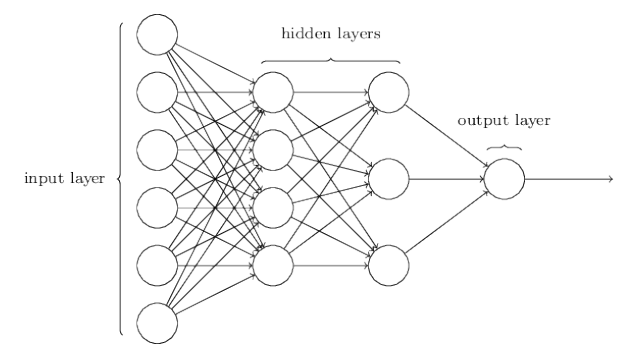
\includegraphics[width=0.65\textwidth]{figures/michael-nielsen-nn-architecture.png}
    \caption{An example of a neural network architecture~\cite{michael-nielsen-nn}}
    \label{fig:nn-example-architecture}
\end{figure}

The difference between \gls{nn} and \gls{cnn} is the among others the architectural blueprint. In \gls{cnn} neurons also have another property: the neurons are arranged in three dimensions: \textcquote{introduction-to-cnn}{the spatial dimensionality of the input(\textbf{height} and the \textbf{width}), and the \textbf{depth}}. The spatial dimensionality is the pixels, and the depth is one, since \gls{mnist} is monochrome.


%Ugly figure and not 100% visual, but it is simple
\begin{figure}[htb!]
    \centering
    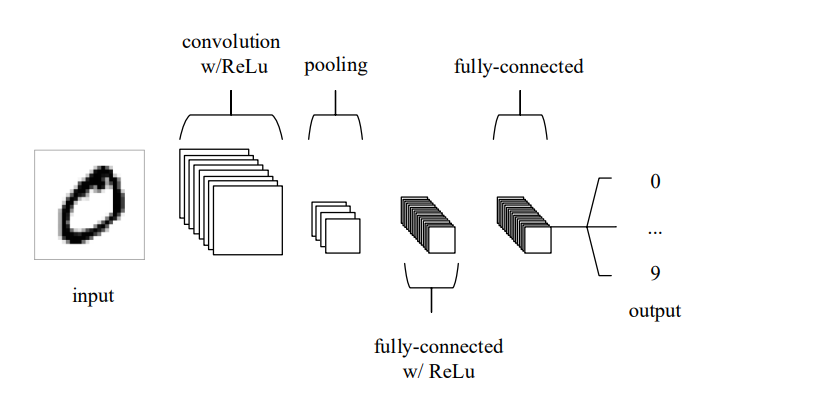
\includegraphics[width=0.8\textwidth]{figures/cnn-simple-architecture.png}
    \caption{An example of a convolutional neural network architecture~\cite{introduction-to-cnn}}
    \label{fig:simple-cnn-architecture}
\end{figure}
%Blog-like structure where CNN is depicted

\gls{cnn}'s architecture constitutes three different types of layers: convolutional layers, pooling layers, and fully-connected layers. The architecture of a \gls{cnn} can be shown in Figure \ref{fig:simple-cnn-architecture}. The convolutional layers \textcquote{introduction-to-cnn}{will determine the output of neurons of which are connected to local regions of the input}, which is also called a convolution. The pooling layers reduce the number of parameters in the previous layers. The fully-connected layers act as normal \gls{nn} layers~\cite{introduction-to-cnn}.


A convolution, as described, acts as a filter which maps the input to an output matrix $conv$ of size $n \times n$. The mapping is done by the elementwise-multiplication of the input matrix with the $conv$ matrix. The operation can be seen in Figure \ref{fig:convolution}. The manner in which such mapping is achieved is by sliding over the input matrix, from left to right, top to bottom, with a $n \times n$ matrix one pixel at a time. For each convolution operation \gls{relu} is applied to the operation, where \gls{relu} is a function which takes the maximum value between 0 and the input~\cite{google-cnn}.

\begin{figure}[htb!]
    \centering
    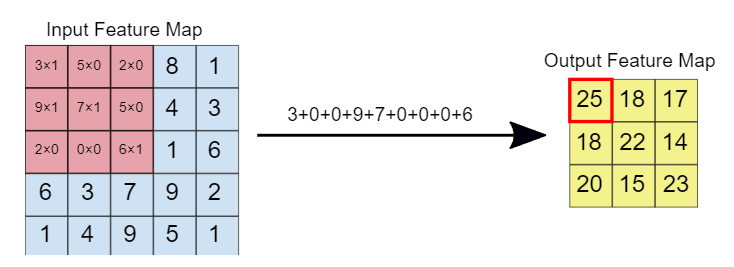
\includegraphics[width=0.7\textwidth]{figures/google-cnn-convolution-example.png}
    \caption{An example of a convolution operation~\cite{google-cnn}}
    \label{fig:convolution}
\end{figure}

In the pooling layer behaves like a convolution, but this time it filters the $conv$ matrix with a $pool$ matrix of size $n \times n$. One method which has been presented~\cite{google-cnn} is the use of max pooling; in the convolutional layer the elementwise multiplication is applied, whereas in max pooling the element with the highest number in the respective matrix is chosen~\cite{google-cnn}. Figure \ref{fig:maxpooling} is provided to show how it works. The pooling layer can be seen as a dimensionality reduction method, because it reduces the data while preserving the original features.

\begin{figure}[htb!]
    \centering
    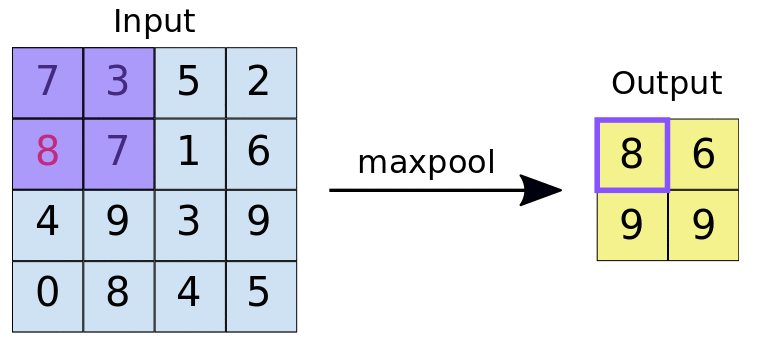
\includegraphics[width=0.5\textwidth]{figures/google-cnn-maxpooling-example.png}
    \caption{An example of a max pooling operation~\cite{google-cnn}}
    \label{fig:maxpooling}
\end{figure}

The last layer is the fully-connected layer, which is connected to all the neurons from the pooling layer. According to Keiron ~\cite{introduction-to-cnn}, the activation function \gls{relu} might be suited to be used in this layer too~\cite{lecun-mnist-database}.

\subsection{Model training}\label{subsec:model-training}
The theory deciding the cross validation methods is described in Chapter~\ref{cha:theory}.



% @book{michael-nielsen-nn,
%   title={Neural networks and deep learning},
%   author={Nielsen, Michael A},
%   volume={25},
%   year={2015},
%   publisher={Determination press San Francisco, CA, USA}
% }
% @misc{faster-svm,
%   doi = {10.48550/ARXIV.1808.06394},
  
%   url = {https://arxiv.org/abs/1808.06394},
  
%   author = {Schlag, Sebastian and Schmitt, Matthias and Schulz, Christian},
  
%   title = {Faster Support Vector Machines},
  
%   publisher = {arXiv},
  
%   year = {2018},
  
%   copyright = {arXiv.org perpetual, non-exclusive license}
% }


% @misc{introduction-to-cnn,
%   doi = {10.48550/ARXIV.1511.08458},
  
%   url = {https://arxiv.org/abs/1511.08458},
  
%   author = {O'Shea, Keiron and Nash, Ryan},
  
%   title = {An Introduction to Convolutional Neural Networks},
  
%   publisher = {arXiv},
  
%   year = {2015},
  
%   copyright = {arXiv.org perpetual, non-exclusive license}
% }


% @misc{mnist-classification-benchmark,
%     url = {https://paperswithcode.com/sota/image-classification-on-mnist},
%     title = {Image Classifcation onf MNIST},
%     year = {2022}
% }

% @misc{google-cnn,
%     organization = {Google},
%     url = {https://developers.google.com/machine-learning/practica/image-classification/convolutional-neural-networks},
%     title = {ML Practicum: Image Classification},
%     year = {2022}
% }

\section{Problem Statement}\label{sec:problem-statement}
\subsection{Audio} 
For models that predict what music is popular or what genre the music is we would like to see how big of an effect feature engineering has for the model. We would like to investigate which kind of dimensionality reduction works best considering both linear and nonlinear aproaches and what they contribute to in the model and when it is a better fit. The performance of these dimensionality reductions is evaluated based on how they affect the performance of the model and their visualisations.

\subsection{Pokemon}
For a model that clasifies Pokemon we would like to see how big of an effect feature engineering has for the model. We would also like to investigate which kind of dimensionality reduction works best and consider both linear and nonlinear aproaches and what they each contribute and when theyre correct to use. The performance of these aproaches might be evaluated based on their visualisations and how they affect model performance.

\subsection{Match data}
For models that predict the outcome of football matches we would like to see how big the effect of feature engineering has for the model. We would also like to investigate which kind of dimensionality reduction works best considering both linear and nonlinear aproaches and what they contribute to in the model and when it is a better fit. The performance of these dimensionality reductions is evaluated based on how they affect the performance of the model and their visualisations.
\chapter{Theory}\label{cha:theory}
This chapter will discuss the theory behind \gls{ml} and \gls{fe}. We will briefly introduce the steps in how the theory will be implemented on a sketch, then describe the theory behind \gls{ml} and \gls{fe}, and then go into more detail about the different methods used in this project on the thoughts behind why choosing them.

\section{Images}\label{sec:images}
As mentioned before, the project will use the \gls{mnist} dataset; the dataset comprises images; therefore, a digital image consists of pixels. In a grayscale image, each pixel has a value between 0 and 255, where 0 is white, and 255 is black. Each pixel has three values in a color image - one for each color: red, green, and blue. The number of pixels in an image is the number of pixels multiplied by the number of colors. For example, a 28x28x1 grayscale image has 784 pixels, while a 28x28x3 color image also has 784 pixels.

In this way, each pixel represents the image's feature (dimension). As the size of images increases, this quickly becomes a large number of features, and for \gls{ml}, it is likely only necessary to use some of them. The process of choosing the most critical features is called feature selection and leads to dimensionality reduction, the topic of this report.

\section{Dimensionality reduction}\label{sec:dimensionality-reduction}
In general, dimensionality reduction transforms data with many features (dimensions) into a new representation of the data with fewer features while preserving as much relevant information as possible. Dimensionality reduction is made by finding a transformation of the data that maps the data to some lower dimensional space while keeping the mean distances between the data points~\cite{dimensionality-reduction-comparative-review}.

Dimensionality reduction can be divided into two categories: linear and nonlinear methods, described in Section \ref{sec:linear-vs-nonlinear}. This section presents some of the standard methods from both categories.

\todo[inline]{Linear methods are based on the assumption that the data is linear. 
A linear dataset is one in which all possible prediction outcomes can be obtained by combinations of the original features without any additional interactions. 
You can show an example of linear data for regression and classification. 
Note that this difference is not so strict as some methods could be thought of as both}


\subsection{Linear methods}\label{subsec:linear-methods}
The linear methods covered are: \gls{pca}, \gls{fa}, \gls{nmf}, and \gls{lda}.


\subsubsection{Principal Components Analysis}\label{subsubsec:principal-components-analysis}
\gls{pca} is a linear method used to reduce a dataset's dimensionality by projecting it onto a lower dimensional subspace, retaining as much of the variance as possible. The best projection is found through the directions of maximum variance in the data based on the covariance matrix and then projecting the data onto those directions. The directions of maximum variance are principal components, and the projection results from the \gls{pca}~\cite{dimensionality-reduction-comparative-review}.


\subsubsection{Factor Analysis}\label{subsubsec:factor-analysis}
\gls{fa} is very similar to \gls{pca}, and \gls{pca} may be called a type of \gls{fa}. However, \gls{fa} is based on the assumption that the data is generated by a linear combination of a few latent variables called factors and that the observed variables are a linear combination of the latent variables plus some noise.

The goal of \gls{fa} is to find the factors that explain the most covariance in the data. Intuitively, related items have stronger mathematical correlations and can thus be grouped with less loss of information. Once the correlations are determined, a rotation is performed to make the factors easier to interpret~\gls{fa}~\cite{decoster-1998-factor-analysis-overview}.


\subsubsection{Non-negative matrix factorization}\label{subsubsec:non-negative-matrix-factorization}
\gls{nmf} constructs approximate factorizations of a non-negative data matrix $V$ into two non-negative matrices $W$ and $H$ such that $V \approx WH$. The non-negativity constraints permit the intuition that data may represent parts forming a whole, which can be thought of as a sum of parts~\cite{lee-1999-learning-nmf}. For example, a text document may represent a combination of topics, and each may represent a combination of words.


\subsubsection{Linear Discriminant Analysis}\label{subsubsec:linear-discriminant-analysis}

\gls{lda} is quite similar to \gls{pca} since they both try to project data into a hyperplane. Still, instead, \gls{lda} tries to maximize class separability, making it easier to contrast classes. \gls{lda} finds the hyperplane with the most separation between the classes and keeps the data points with the same class as close together as possible. This is a three-step process. The first step is to determine the separation between different classes (between-class variance) as the distance between the means of each class. Secondly, the distance between the mean and samples of each class (within-class variance) is calculated. The third step is creating a lower dimensional representation that maximizes the between-class variance and minimizes the within-class variance~\cite{linear-discriminant-analysis-tutorial}.


\subsection{Non-linear methods}\label{subsec:non-linear-methods}
Sometimes high-dimensional data may contain non-linear relationships, which linear methods cannot capture. It has been shown that \gls{pca} fails to find significant components in the swiss-roll dataset~\cite{tennenbaum}. In such cases, non-linear methods are used. The non-linear methods covered are \gls{kpca}, \gls{mds}, and \gls{isomap}.


\subsubsection{Kernel Principal Component Analysis}\label{subsubsec:kernel-principal-component-analysis}
\gls{kpca} is an extension of \gls{pca}, and it projects the data onto a higher dimensional plane, where \gls{pca} is performed. 
The first step is to construct the kernel matrix from the data. The kernel matrix is a matrix of the dot products of the data points, the kernel matrix is used like the covariance matrix in \gls{pca}~\cite{kernel-pca}. In the kernel matrix the data is in a higher dimensional space, where the data is linear separable. By using the kernel function, \gls{kpca} exposes the kernel trick, which is instead of calculating the dat into a higher dimensional space, it calculates the inner product between the datapoints, which is computationally cheap to calculate instead of calculating every datapoint into a higher dimensional space.
The kernel matrix is then centered by subtracting the mean of each row and column. This matrix is also called the Gram matrix. The Gram matrix is then used to find eigenvectors and eigenvalues. By using the kernel trick, \gls{kpca} can compute eigenvalue decomposition, as in \gls{pca}.The eigenvectors are then used to project the data onto a higher dimensional space, where \gls{pca} is performed. The eigenvectors with the highest eigenvalues are the principal components, and the projection is the data projected onto the principal components~\cite{kernel-pca}. 

\subsubsection{Isometric Feature Mapping}\label{subsubsec:isometric-feature-mapping}
\gls{isomap} is another non-linear method that is a special case of \gls{cmds}. It is assumed that \gls{isomap} is suited to discover manifolds of arbitrary dimensionality and that it guarantees an approximation of the true structure of the manifold~\cite{tennenbaum}.

The first step in \gls{isomap} is to map the data points in a graph. The graph is constructed by connecting each point to its nearest neighbors. The user sets the number of nearest neighbors. The nearest neighbors are found by using the Euclidean distance. The Euclidean distance is the linear distance between two points in a Euclidean space~\cite{Multidimensional-Scaling-Sammon-Mapping-and-Isomap}.

In the second step, \gls{isomap} finds the Geodesic distance between each point~\cite{Multidimensional-Scaling-Sammon-Mapping-and-Isomap}. The Geodesic distance is the shortest distance between two points on the surface of a sphere. The Geodesic distance is calculated by finding the shortest path between two points on a graph. The graph is constructed by connecting each point to its nearest neighbors. The shortest path can be found by using the Dijkstra algorithm~\cite{multi-dimensional-scaling-leeuw}.

The final step in \gls{isomap} is finding the data's \gls{mds} projection. The \gls{mds} projection is found by minimizing the stress function. The stress function is the sum of the squared differences between the distances in the original data and the distances in the projected data~\cite{multi-dimensional-scaling-leeuw}, so the stress function finds the slightest change in the data. The minimum of this stress function will be the best reproduction of the data in lower dimensional space according to the \gls{isomap} algorithm. 



\subsection{Choice of dimensionality reduction}
Four different dimensionality reduction methods have been chosen to be in the implementation. These are linear and nonlinear methods, particularly \gls{pca}, \gls{lda}, \gls{kpca}, and \gls{isomap}. The group chose these four because they cover the spectrum of options well and are some of the most used. Only four were selected to keep the project's focus tight and the right amount of depth versus breadth of the project.

%ISOMAP 


%The geodesic distance is used in \gls{isomap} to find the shortest distance between two points in a dataset. %These will be clarified first before clarifying \gls{isomap}. 

%\subparagraph{Multi Dimensional Scaling}\label{subsec:multi-dimensional-scaling}
%\gls{mds} is a non-linear method that is used to reduce the dimensionality of a dataset by projecting it onto a lower dimensional subspace, while preserving as much of the variance between the data as possible. The projection is found by calculating the best result from the \gls{mds} function which is a modified version of the STRESS function. The STRESS function finds the least change in data when in the case of \gls{mds} is when reducing the dimensionality~\cite{multi-dimensional-scaling-leeuw}.

%\subparagraph{Geodesic distance}\label{subsec:geodesic-distance}
%Geodesic is a distance between two points on a surface of a sphere. The geodesic distance between two points is the shortest distance between the two points on the surface of a sphere. The geodesic distance is calculated by finding the shortest path between two points on a graph. The graph is constructed by connecting each point to its nearest neighbors. The shortest path is found by using the Dijkstra's algorithm~\cite{multi-dimensional-scaling-leeuw}.


% In this project we will focus on dimensionality reduction for the purpose of computer vision, and in particular for the MNIST dataset.


% In this project we will study some common methods of dimensionality reduction using the MNIST dataset for digit recognition.
\section{Evaluation and metrics}\label{sec:evalueation}

A pipeline is generally evaluated based on quantitative metrics in machine learning and data science. These metrics are in classification general based on the confusion matrix. An example of a confusion matrix can be seen in \todo{need to make pictue}. It represents all the guesses a ml model has made, where the x-axis, in this case, is the true class of a given data point, and the y-axis is the class the model has guessed the data point to have. The numbers are how many times the model has guessed the different combinations. \cite{james-statistical-learning}

\subsection*{Metrics}

There exist many metrics, but generally, there are four basic metrics. These are accuracy, precision, recall, and f1. Outside these, there are more esoteric metrics like the Mattheus correlation coefficient, Cohen's kappa, and more. The following section will describe each of the four basic metrics. \cite{metrics-for-multi}

Accuracy is the most straightforward of the metrics. It describes the percentage of correct guesses out of all guesses. This metric works well in cases where the sizes of the different classes are similar. It struggles in cases where one class is much larger than another. Here It is possible to achieve very high accuracy by only guessing the larger class, which can make a model seem impressive while simultaneously not doing what it is supposed to if it is crucial to find the smaller class.

In the case where one class is smaller is where the precision metric comes in handy. It is calculated by taking the correct guesses for a class and dividing them by all guesses on this class, which includes wrong guesses. This gets around the problems accuracy has with classes with very different sizes because it is not possible to always guess the bigger class and get a good precision.

The third metric is recall, primarily used in cases where it really matters if one class is guessed correctly. Recall could be in cases like corona, where a false positive is much better than a false negative. Recall is calculated by dividing the true positives by true positives and false negatives.

The last basic metric is f1. Its commonly used when both recall and precision are essential. It is calculated two times precision times recall decided by precision plus recall.


In a pipeline, these metrics are generally used for hyperparameter tuning and general evaluation of the model's performance. Here hyperparameter tuning will generally only use a single metric to focus on to maximize it. In evaluation, on the other hand, the metrics are used more generally to explain what the model does well and what it does not do well. \cite{james-statistical-learning}

% @book{poynton2012digital,
%   title={Digital Video and HD: Algorithms and Interfaces},
%   author={Poynton, C.},
%   isbn={9780123919328},
%   year={2012},
% }

\chapter{Implementation}\label{cha:implementation}
This chapter covers the implementation details for the project. The implementation is created in python 3.8.10 and uses the \glsfirst{sklearn} library for the machine learning algorithms.


The chapter starts with an overview of the pipeline used for the project based on the considerations from \autoref{cha:theory}; this is followed by the essential implementation details and the machine learning algorithms, from pre-processing to hyperparameter tuning.

\section{Pipeline overview}\label{sec:pipeline-overview}
The development for this project is an extension of the general pipeline from \autoref{fig:basic-machine-learning-pipeline} extended with the considerations from \autoref{cha:theory}.

\autoref{fig:pipeline-overview} shows an overview of the developed pipeline, which consists of five segments: The dataset, the pre-processing, the dimensionality reduction, the machine learning loop, and the output.


\begin{figure}[b!]
    \centering
    \begin{tikzpicture}[node distance=1.5cm, auto, every node/.style={scale=0.7}]
    %MNIST Original logo
    \node (db-slice1) [cylinder, shape border rotate=90, draw, minimum height=1cm,minimum width=3.32cm, aspect=1.1] {};
    \node (db-slice2) [cylinder, shape border rotate=90, draw, minimum height=1cm,minimum width=3.32cm, text centered, above=0pt of db-slice1.before top, anchor=after bottom,aspect=0.1] {MNIST original};
    \node (db-slice3) [cylinder, shape border rotate=90, draw, minimum height=1cm,minimum width=3.32cm, above=0pt of db-slice2.before top, anchor=after bottom, aspect=1.1] {};

    %MNIST Argumented logo
    \node (db-slice4) [cylinder, shape border rotate=90, draw, minimum height=1cm,minimum width=3.7cm, aspect=1.4, shift={($(db-slice1.south)+(0cm,-4.5cm)$)}] {};
    \node (db-slice5) [cylinder, shape border rotate=90, draw, minimum height=1cm,minimum width=3.7cm, text centered, above=0pt of db-slice4.before top, anchor=after bottom,aspect=0.1] {MNIST augmented};
    \node (db-slice6) [cylinder, shape border rotate=90, draw, minimum height=1cm,minimum width=3.7cm, above=0pt of db-slice5.before top, anchor=after bottom, aspect=1.4] {};

    \node (a) [cluster, shift={($(db-slice2.east)+(2cm,-2.5cm)$)}] {pre-processing};
    \node (b) [cluster, shift={($(a.east)+(4cm,0cm)$)}] {No dimensionality reduction};
    \node (c) [cluster, below of=b] {Dimensionality reduction};
    \node (d) [circle, shift={($(c.south west)+(0.5cm,-2.5cm)$)}] {Linear};
    \node (e) [circle, shift={($(c.south east)+(-0.5cm,-2.5cm)$)}] {Non linear};
    \node (f) [cluster, shift={($(b.east)+(3.5cm,0cm)$)}] {Machine learning model};
    \node (g) [cluster, below of=f] {output};

    \node (o) [shift={($(a.west)+(-2cm,0cm)$)}] {};
    \node (p) [shift={($(a.east)+(0.5cm,0cm)$)}] {};
    \node (q) [shift={($(b.east)+(0.5cm,0cm)$)}] {};

    \draw [arrow, -] (db-slice1.south) -- ++(0,0) -| (o.west);
    \draw [arrow, -] (db-slice6.north) -- ++(0,0) -| (o.west);
    \draw [arrow, ->] (o.west) -- (a.west);

    \draw [arrow, ->] (a.east) -- (b.west);
    \draw [arrow, ->] (p.east) -- ++(0,-1) |- (c.west);

    \draw [arrow, -] (c.south) -- ++(0,-0.75) -| (e.north);
    \draw [arrow, -] (c.south) -- ++(0,-0.75) -| (d.north);

    \draw [arrow, ->] (b.east) -- (f.west);
    \draw[arrow, ->] (f) to[loop above,looseness=9] node[above,scale=0.8, xshift=-10,yshift=7] {We train the model with the training data} (f);
    \draw [arrow, -] (c.east) -- ++(0,0) -| (q.east);
    \draw [arrow, ->] (f.south) -- (g.north);
\end{tikzpicture}
    \caption{Overview of the pipeline used for the project.}
    \label{fig:pipeline-overview}
\end{figure}


The first segment, the dataset, covers downloading the dataset, loading it into the program, and augmenting the original dataset to create a new one.

The second segment, pre-processing, covers reshaping the data into a form usable with the \gls{sklearn} library and scaling the data in preparation for the next segment.

The third segment, and the focus of this project, is dimensionality reduction. This segment consists of the four dimensionality reduction algorithms: \gls{pca}, \gls{lda}, \gls{isomap}, and \gls{kpca}, as well as no dimensionality reduction.

The fourth segment is the tuning loop, where grid search with cross-validation determines the best hyperparameters for the \gls{svm} based on the f1-score. Because the project focuses on dimensionality reduction, this loop includes the number of components for dimensionality as a hyperparameter as well.

Finally, the fifth segment is the output. Once the best hyperparameters are determined, the \gls{svm} is trained on the whole dataset and tested on the test set. The results of the grid search - scores, parameters, and scoring time - and the results of the final \gls{svm} - confusion matrix and classification report - are saved.

\section{Pipeline implementation}\label{sec:pipeline-implementation}
This section presents the project's implementation details per the descriptions from \autoref{sec:pipeline-overview}.

\subsection{Data and pre-processing}\label{subsec:data-and-pre-processing}
The \gls{mnist} dataset is downloaded from \url{http://yann.lecun.com/exdb/mnist/}\cite{lecun-mnist-database} and loaded into the program using the idx2numpy library. It was later discovered that the \gls{sklearn} library has a built-in function for downloading the MNIST dataset, but this was not discovered until after the dataset was downloaded manually.

The data is comprised of four parts. The training images (\texttt{X}), training labels (\texttt{y}), test images (\texttt{X\_test}), and test labels (\texttt{y\_test}).


\begin{listing}[htb!]
    \centering
    \begin{minted}{python}
        load_mnist() # helper function for downloading the MNIST dataset
        X = idx2numpy.convert_from_file(
        'src/mnist_data/train_file_image').reshape(60000, 784)
        y = idx2numpy.convert_from_file('src/mnist_data/train_file_label')
        X_test = idx2numpy.convert_from_file(
        'src/mnist_data/test_file_image').reshape(10000, 784)
        y_test = idx2numpy.convert_from_file('src/mnist_data/test_file_label')
    \end{minted}
    \caption{Data segment of pipeline details.}
    \label{lst:data-segment}
\end{listing}


Each image is reshaped from a 28x28 matrix to a 784x1 vector, which is the input that \gls{sklearn} expects. If the pipeline was followed strictly, this reshaping should be done in the pre-processing segment, but it was done here for convenience.

\subsection{Tuning loop}\label{subsec:tuning-loop}
The last part of the pre-processing segment and the remaining segments of the pipeline are implemented together, where each dimensionality reduction method has its own function as per \autoref{sec:pipeline-overview}. There are five functions in total, one for each dimensionality reduction method and one for no dimensionality reduction. The baseline \gls{svm} function is shown in \autoref{lst:baseline-svm-results} with comments in the code highlighting the differences between the functions.


\begin{listing}[htb!]
    \centering
    \begin{minted}{python}
        def baseline_svm_results(X, y, X_test, y_test, hyperparameters, methodname="baseline_svm"):
            baseline_model_pipeline = Pipeline(steps=[
                ("scaler", StandardScaler()),
                # ("dimensionality_reduction", PCA()/LDA()/ISOMAP()/KernelPCA),
                ("classifier", SVC(kernel="linear", decision_function_shape="ovo", random_state=42))])
            search = GridSearchCV(baseline_model_pipeline,
                                hyperparameters,
                                cv=5,
                                scoring="f1_macro",
                                verbose=10,
                                n_jobs=-1) # -1 uses all available cores. The nonlinear methods are limited to 1 core
            search.fit(X, y)
            y_pred = search.best_estimator_.predict(X_test)
            save_results(methodname, # Helper function for saving results
                 search.cv_results_, # Save csv with gridsearch results
                 ConfusionMatrixDisplay(confusion_matrix(y_test, y_pred)), # Save confusion matrix
                 classification_report(y_test, y_pred, output_dict=True)) # Save classification report
    \end{minted}
    \caption{The baseline implementation of the tuning loop. The hyperparameters are passed as a dictionary. The \texttt{methodname} parameter is used for naming the output files.}
    \label{lst:baseline-svm-results}
\end{listing}


The functions use the \gls{sklearn} library's \texttt{Pipeline} class to create a pipeline of the pre-processing, dimensionality reduction, and classifier steps. As per \autoref{sec:pipeline-overview}, the pre-processing step is a standard scaler. The dimensionality step depends on the function and is either \gls{pca}, \gls{lda}, \gls{isomap}, or \gls{kpca}. The classifier step is a support vector machine with a linear kernel and one-versus-one decision function shape and a random state of 42. The random state is used to ensure that the results are reproducible.

The classifier could be built using different \gls{sklearn} functions as well, which could have improved performance. Using the \texttt{LinearSVC()} and \texttt{OneVsOneClassifier()} functions might have been more correct that the current implementation, however the way it is implemented now would allow us to use a different kernel for the \gls{svm} defined through the hyperparameter dictionary.

The \texttt{GridSearchCV} class is used to perform the hyperparameter tuning. The \texttt{GridSearchCV} class takes a pipeline as input and a dictionary of hyperparameters. Additionally the implementation sets the cross-validation number, a scoring function, a verbosity level, and the number of cores to use.

cv is the cross-validation number, in which grid search performs non-shuffled stratified k-fold cross-validation with 5 folds. The scoring function is the f1 macro score, which is the harmonic mean of the precision and recall. The verbosity level is set to 10, which means that the progress of the grid search is printed to the console in high detail. The number of cores is set to -1, which means that all available cores are used. The nonlinear methods are limited to 1 core, because of computational limits - the nonlinear methods use a lot more memory than the linear methods, which causes the program to crash if too many cores are used.


The functions are similar in structure, but they use a different number of cores and are called with a different set of hyperparameters.

\subsubsection{The hyperparameters}\label{subsubsec:the-hyperparameters}
The following hyperparameters are used for the tuning loop:


\begin{listing}[htb!]
    \centering
    \begin{minted}{python}
        c_logspace = np.logspace(-3, 0, 4)
        gamma_logspace = np.logspace(-3, 0, 4)
        svm_hyperparameters = {
                "classifier__C": c_logspace, }
        pca_hyperparameters = {"pca__n_components": [9, 16, 25, 36, 49],}
        lda_hyperparameters = {"lda__n_components": [5, 6, 7, 8, 9],}
        isomap_hyperparameters = {
            "isomap__n_components": [4, 9, 36, 49],
            "isomap__n_neighbors": [4, 5],}
        kernel_pca_hyperparameters = {
            "kernel_pca__n_components": [36, 49],
            "kernel_pca__gamma": gamma_logspace,
            "kernel_pca__kernel": ["rbf", "sigmoid"]}
    \end{minted}
    \caption{Hyperparameters used in the tuning loops.}
    \label{lst:hyperparameters-dictionaries}
\end{listing}


The dictionaries are combined into single dictionaries for use in the results functions. For example, the \gls{svm} hyperparameters are combined with \gls{pca} hyperparameters to create a full hyperparameter dictionary for that method.

With regards to the hyperparameters that are shown in~\ref{lst:hyperparameters-dictionaries}, the reason for choosing the values is explained in the remainder of this section.


\gls{svm} has one hyperparameter, the regularization parameter C, which penalizes the model when a sample is misclassified. The default value is 1, and higher values for C will improve the model's ability to classify the samples correctly~\cite{scikit-learn}. The group chose to use a logarithmic space between 0.001 and 1 to see how much the regularization parameter affects the results. \gls{lda} can only be used with up to nine components, as compared to the other methods. \gls{isomap} has the number of neighbors as hyperparameter, which is the number of points for the k-nearest neighbors used in \gls{isomap}. In the default implementation the number five is used~\cite{scikit-learn}. The gamma hyperparameter for \gls{kpca} is a constant which is used to calculate the kernel function. The group chose values under 1 because, according to sklearn, a recommended value is 1 divided by the number of features~\cite{scikit-learn}. The default kernel, which is presented, is the \gls{rbf} kernel. Another different kernel is the sigmoid kernel, which projects the data onto a sigmoid curve. 



% Template for a listing
% \begin{listing}[htb!]
%     \centering
%     \begin{minted}{python}
%         print("hello World")
%     \end{minted}
%     \caption{}
%     \label{lst:}
% \end{listing}
\chapter{Results}\label{cha:results}
This chapter presents the results of the project. The results are presented in the form of experiments, all experiments are based on the hypothesis: \begin{quote}
    Nonlinear dimensionality reduction methods work as well as linear methods on the \gls{mnist} dataset
\end{quote}
The results are presented in the form of tables and a figures for each experiment. The table shows the results of the experiment and the figure shows the results of the experiment in a visual manner.  The experiments are presented in the following order:
\begin{enumerate}
    \item \textbf{Experiment 1:} What dimensionality reduction methods work best on the \gls{mnist} dataset, when used best?
    \item \textbf{Experiment 2:} How many dimensions can a method reduce before a significant loss of accuracy occurs?
    \item \textbf{Experiment 3:} What impact does Kernels and hyperparameters have on the dimensionality reduction methods?
    \item \textbf{Experiment 4:} What happens with the dimensionality reduction when the amount of data is reduced, do they still hold for hypothesis?
\end{enumerate}


\section{Experiment 1}\label{sec:experiment-1}
%Needs an introduction to the experiment, and why it is relevant to the problem statement.
% relevance to problem anal. and introduction (why is this relavant)
The problem statement states to find the impact of dimensionality reduction, comparing linear and nonlinear methods. This experiment compares the chosen dimensionality reduction methods in each of their best configurations on the chosen MNIST dataset. This experiment is relevant to the problem statement, as it is the first step in finding the impact of dimensionality reduction. The experiment is also relevant to the problem analysis, as it explores the impact of dimensionality reduction in ML. The experiment also finds the best configuration for each method was essential to comparing the methods on the same number of samples.



\subsection{Rules and overview of experiment}\label{subsec:experiment-1-rules}
% Rules and what have we done, how do we evaluate (write about specs here)
The dimensionality reduction methods used in the experiment were \gls{svm}, \gls{pca}, \gls{lda}, \gls{kpca}, and \gls{isomap}. The baseline SVM ML model was also used without any dimensionality reduction. Each method was first cross-validated, finding the best hyperparameters for 15000 samples. Every method was tested with the same number of components. Besides LDA, it can only use up to 9 components. Then some of the methods were cross-validated again with 60000 samples to find how the methods performed with more data; the same components were still used. The methods tested on 60000 samples were the baseline SVM, PCA, and LDA, as the computer used in the experiment could not handle kPCA and ISOMAP with 60000 samples of data. The configurations used for each are shown in Table \ref{tab:best-configuration}.

\begin{table}[htb!]   
    \centering
    \begin{tabular}{lrlll}
        \toprule
        method & components & C & parameter & parameter\\
        \midrule
        SVM-15 & 784 & C = 0.01 &  \\
        SVM-60 & 784 & C = 0.01 &  \\
        LDA-15 & 9 & C = 0.1 &  \\
        LDA-60 & 9 & C = 1.0 &  \\
        PCA-15 & 49 & C = 0.01 &  \\
        PCA-60 & 49 & C = 0.1 &   \\
        KPCA-15 & 49 & C = 1.0 & Gamma = 0.01 & Sigmoid \\
        ISOMAP-15 & 49 & C = 0.001 & neighbours = 5 \\
        \bottomrule
    \end{tabular}
    \caption{Best configuration for each method used for experiment-1, method-15 and method-60, means the method with 15 and 60 thousand samples.}
    \label{tab:best-configuration}
\end{table}

Every test in experiment 1 was made on the same computer, namely pc-2. See \autoref{tab:pc-specs} for the specific specs for the comuter used in the experiment. 

The experiment results are shown in \autoref{subsec:experiment-1-results}. The results are in the form of classification reports and confusion matrixes, which show the precision, recall, f1-score, support for each class, and the total accuracy for each method. The methods will be compared in accuracy, f1-score, and time fitting the data.

\subsection{Results}\label{subsec:experiment-1-results}
% Show results (desribe the most relavant results)
Below is shown the results for the methods. The results are in the form of classification reports, which show the precision, recall, f1-score, support for each class, and the total accuracy for each method. The methods will be compared in accuracy, f1-score, and time fitting the data. 

\begin{table}[htb!]
\centering
\begin{tabular}{lrrrr}
\toprule
 & precision & recall & f1-score & support \\
\midrule
0 & 94.7886 & 98.3673 & 96.5448 & 980 \\
1 & 96.3979 & 99.0308 & 97.6967 & 1135 \\
2 & 92.2488 & 93.4109 & 92.8262 & 1032 \\
3 & 90.8203 & 92.0792 & 91.4454 & 1010 \\
4 & 93.4739 & 94.8065 & 94.1355 & 982 \\
5 & 90.7940 & 88.4529 & 89.6082 & 892 \\
6 & 95.6705 & 94.5720 & 95.1181 & 958 \\
7 & 94.4828 & 93.2879 & 93.8815 & 1028 \\
8 & 93.1842 & 89.8357 & 91.4794 & 974 \\
9 & 92.8717 & 90.3865 & 91.6123 & 1009 \\
accuracy & & & 93.5400 & 10000 \\
macro avg & 93.4733 & 93.4230 & 93.4348 & 10000 \\
weighted avg & 93.5263 & 93.5400 & 93.5199 & 10000 \\
\bottomrule
\end{tabular}
\caption{Classification report for baseline\_svm\_15000}
\label{tab:classification-report-baseline_svm_15000}
\end{table}
 %37
\begin{figure}[htb!]
    \centering
    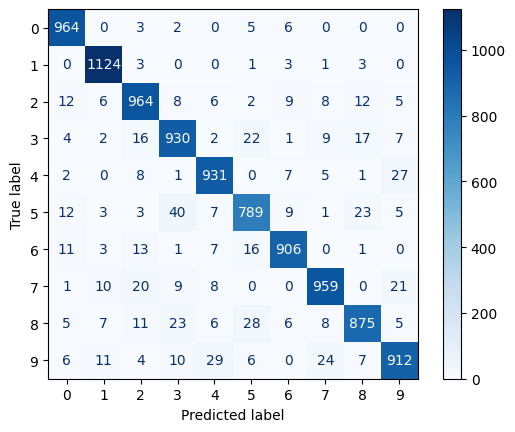
\includegraphics[width=0.8\textwidth]{figures/1-experiment/confusion_matrix_baseline_svm_15000.png}
    \caption{Confusion matrix for baseline SVM with 15000 samples.}
    \label{fig:confusion-matrix-baseline_svm_15000}
\end{figure}
\subsubsection{\gls{svm} with 15000 samples}\label{subsubsec:experiment-1-results-svm-15000}
Table \ref{tab:classification-report-baseline_svm_15000} shows the accuracy for \gls{svm} without any dimensionality reduction with 15000 samples. The accuracy is 93.54\%, and it takes 37 seconds to train the model. \autoref{fig:confusion-matrix-baseline_svm_15000} shows \gls{svm} is best at recognizing zeros and one's in pictures, as the model has the f1-score in these classes, with the scores 96.5\% and 97.7\%. The model has some trouble recognizing fives, eights, and threes, as these are the lowest scoring in the f1-score for all the classes, with five being 89.6\%, eight being 91.5\%, and three being 91.4\%. With an average f1-score of 93.43\%, the baseline \gls{svm} with 15000 samples is a good model. 

\subsubsection{\gls{svm} with 60000 samples}\label{subsubsec:experiment-1-results-svm-60000}
\begin{table}[htb!]
\centering
\begin{tabular}{lrrrr}
    \toprule
    & precision & recall & f1-score & support \\
    \midrule
    0 & 96.0278 & 98.6735 & 97.3327 & 980 \\
    1 & 97.3958 & 98.8546 & 98.1198 & 1135 \\
    2 & 93.6538 & 94.3798 & 94.0154 & 1032 \\
    3 & 91.6587 & 94.6535 & 93.1320 & 1010 \\
    4 & 93.8124 & 95.7230 & 94.7581 & 982 \\
    5 & 92.4138 & 90.1345 & 91.2599 & 892 \\
    6 & 96.2105 & 95.4071 & 95.8071 & 958 \\
    7 & 95.6262 & 93.5798 & 94.5919 & 1028 \\
    8 & 93.4668 & 91.0678 & 92.2517 & 974 \\
    9 & 94.8012 & 92.1705 & 93.4673 & 1009 \\
    accuracy & & & 94.5600 & 10000\\
    macro avg & 94.5067 & 94.4644 & 94.4736 & 10000 \\
    weighted avg & 94.5599 & 94.5600 & 94.5481 & 10000 \\
    \bottomrule
\end{tabular}
\caption{Classification report for baseline\_svm\_60000}
\label{tab:classification-report-baseline_svm_60000}
\end{table}
 %378
% \begin{figure}[htb!]
%     \centering
%     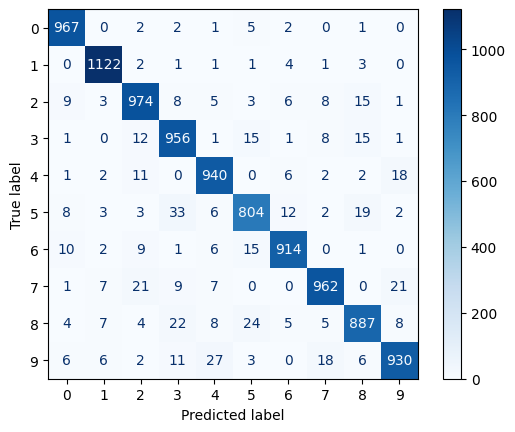
\includegraphics[width=0.8\textwidth]{figures/1-experiment/confusion_matrix_baseline_svm_60000.png}
%     \caption{Confusion matrix for baseline SVM with 60000 samples.}
%     \label{fig:confusion-matrix-baseline_svm_60000}
% \end{figure}
Table \ref{tab:classification-report-baseline_svm_60000} shows the accuracy for \gls{svm} without any dimensionality reduction with 60000 samples. The accuracy is 94.56\% for 60000 samples, and it takes 378 seconds to train the model, which is 6 minutes and 16 seconds. The \gls{svm} model is best at recognizing zeros and ones in pictures, as the model has the f1-score in these classes, with scores of 97.3\% and 98.1\%. The model has some trouble recognizing fives, eights, and threes, as these are the lowest scoring in the f1-score for all the classes, with five being 91.2\%, eight being 92.3\%, and three being 93.1\%. With an average f1-score of 94.47\%, the baseline \gls{svm} with 15000 samples is a good model that uses a significant amount of time.

\subsubsection{\gls{lda} with 15000 samples}\label{subsubsec:experiment-1-results-lda-15000}
\begin{table}[htb!]
\centering
\begin{tabular}{lrrrr}
    \toprule
    & precision & recall & f1-score & support \\
\midrule
0 & 93.1238 & 96.7347 & 94.8949 & 980 \\
1 & 94.3869 & 96.2996 & 95.3336 & 1135 \\
2 & 89.2246 & 85.8527 & 87.5062 & 1032 \\
3 & 85.1781 & 87.6238 & 86.3836 & 1010 \\
4 & 86.9650 & 91.0387 & 88.9552 & 982 \\
5 & 83.6549 & 82.6233 & 83.1359 & 892 \\
6 & 92.1466 & 91.8580 & 92.0021 & 958 \\
7 & 90.3353 & 89.1051 & 89.7160 & 1028 \\
8 & 83.2804 & 80.8008 & 82.0219 & 974 \\
9 & 87.7193 & 84.2418 & 85.9454 & 1009 \\
accuracy & & & 88.7600 & 10000 \\
macro avg & 88.6015 & 88.6178 & 88.5895 & 10000 \\
weighted avg & 88.7285 & 88.7600 & 88.7240 & 10000 \\
\bottomrule
\end{tabular}
\caption{Classification report for lda svm 15000}
\label{tab:classification-report-lda_svm_15000}
\end{table}
 %7
\begin{figure}[htb!]
    \centering
    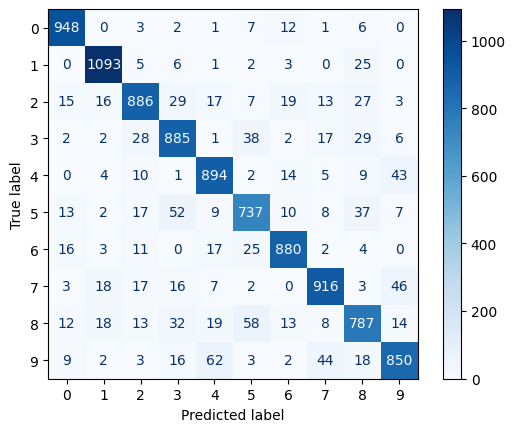
\includegraphics[width=0.8\textwidth]{figures/1-experiment/confusion_matrix_lda_svm_15000.png}
    \caption{Confusion matrix for LDA with 15000 samples.}
    \label{fig:confusion-matrix-lda-15000}
\end{figure}
Table \ref{tab:classification-report-lda_svm_15000} shows the accuracy for \gls{svm} with \gls{lda} as dimensionality reduction with 15000 samples. The accuracy is 88.76\% for 15000 samples, and it takes 7 seconds to train the model. \autoref{fig:confusion-matrix-lda-15000} \gls{svm} model is best at recognizing zeros and ones in pictures, as the model has the f1-score in these classes, with scores of 94.9\% and 95.3\%. The model has some trouble recognizing fives, eights, and nines, as these are the lowest scoring in the f1-score for all the classes, with five being 83.1\%, eight being 82.0\%, and three being 85.9\%. With an average f1-score of 88.59\%, the baseline \gls{svm}with 15000 samples is a worse model but is much faster than simply using \gls{svm}.
\subsubsection{\gls{lda} with 60000 samples}\label{subsubsec:experiment-1-results-lda-60000}
\begin{table}[htb!]
\centering
\begin{tabular}{lrrrr}
    \toprule
    & precision & recall & f1-score & support \\
    \midrule
0 & 93.1953 & 96.4286 & 94.7844 & 980 \\
1 & 94.7232 & 96.4758 & 95.5914 & 1135 \\
2 & 90.0398 & 87.5969 & 88.8016 & 1032 \\
3 & 85.9804 & 86.8317 & 86.4039 & 1010 \\
4 & 88.0929 & 92.6680 & 90.3226 & 982 \\
5 & 84.4318 & 83.2960 & 83.8600 & 892 \\
6 & 91.0387 & 93.3194 & 92.1649 & 958 \\
7 & 90.7093 & 88.3268 & 89.5022 & 1028 \\
8 & 84.9520 & 81.7248 & 83.3072 & 974 \\
9 & 88.4892 & 85.3320 & 86.8819 & 1009 \\
accuracy & & & 89.3300 & 10000 \\
macro avg & 89.1653 & 89.2000 & 89.1620 & 10000 \\
weighted avg & 89.2917 & 89.3300 & 89.2903 & 10000 \\
\bottomrule
\end{tabular}
\caption{Classification report for lda svm 60000}
\label{tab:classification-report-lda_svm_60000}
\end{table}
 %58
% \begin{figure}[htb!]
%     \centering
%     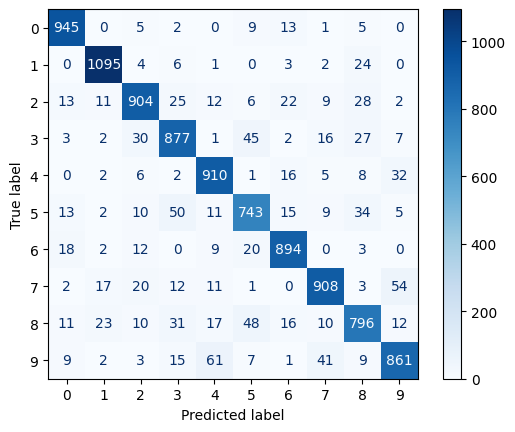
\includegraphics[width=0.8\textwidth]{figures/1-experiment/confusion_matrix_lda_svm_60000.png}
%     \caption{Confusion matrix for LDA with 60000 samples.}
%     \label{fig:confusion-matrix-lda-60000}
% \end{figure}
Table \ref{tab:classification-report-lda_svm_60000} shows the accuracy for \gls{svm} with \gls{lda} as dimensionality reduction with 60000 samples. The accuracy is 89.33\% for 60000 samples, and it takes 58 seconds to train the model. The \gls{svm} model is best at recognizing zeros and ones in pictures, as the model has the f1-score in these classes, with scores of 94.8\% and 95.6\%. The model has some trouble recognizing fives, eights, and threes, as these are the lowest scoring in the f1-score for all the classes, with five being 83.9\%, eight being 83.3\%, and three being 86.4\%. \gls{svm} using \gls{pca} as the dimensionality reduction method has an average f1-score of 89.16\%.

\subsubsection{\gls{pca} with 15000 samples}\label{subsubsec:experiment-1-results-pca-15000}
\begin{table}[htb!]
\centering
\caption{Classification report for pca_svm_15000}
\label{tab:classification-report-pca_svm_15000}
\begin{tabular}{lrrrr}
\toprule
 & precision & recall & f1-score & support \\
\midrule
0 & 0.944773 & 0.977551 & 0.960883 & 980.000000 \\
1 & 0.967938 & 0.984141 & 0.975972 & 1135.000000 \\
2 & 0.904306 & 0.915698 & 0.909966 & 1032.000000 \\
3 & 0.897335 & 0.900000 & 0.898665 & 1010.000000 \\
4 & 0.916914 & 0.943992 & 0.930256 & 982.000000 \\
5 & 0.889143 & 0.872197 & 0.880589 & 892.000000 \\
6 & 0.951832 & 0.948852 & 0.950340 & 958.000000 \\
7 & 0.923002 & 0.921206 & 0.922103 & 1028.000000 \\
8 & 0.904963 & 0.879877 & 0.892244 & 974.000000 \\
9 & 0.927083 & 0.882061 & 0.904012 & 1009.000000 \\
accuracy & 0.923700 & 0.923700 & 0.923700 & 0.923700 \\
macro avg & 0.922729 & 0.922558 & 0.922503 & 10000.000000 \\
weighted avg & 0.923513 & 0.923700 & 0.923467 & 10000.000000 \\
\bottomrule
\end{tabular}
\end{table}
 %10
\begin{figure}[htb!]
    \centering
    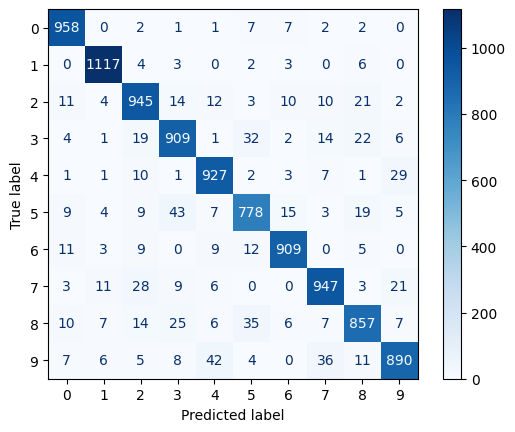
\includegraphics[width=0.8\textwidth]{figures/1-experiment/confusion_matrix_pca_svm_15000.png}
    \caption{Confusion matrix for PCA with 15000 samples.}
    \label{fig:confusion-matrix-pca-15000}
\end{figure}
Table \ref{tab:classification-report-pca_svm_15000} shows the accuracy for \gls{svm} with \gls{pca} as dimensionality reduction with 15000 samples. The accuracy is 92.37\% for 15000 samples, and it takes 10 seconds to train the model. \autoref{fig:confusion-matrix-pca-15000} \gls{svm} model is best at recognizing zeros and ones in pictures, as the model has the f1-score in these classes, with scores of 96.1\% and 97.6\%. The model has some trouble recognizing fives, eights, and threes, as these are the lowest scoring in the f1-score for all the classes, with five being 88.1\%, eight being 89.2\%, and three being 89.9\%. \gls{svm} using \gls{pca} as the dimensionality reduction method has an average f1-score of 92.25\%.

\subsubsection{\gls{pca} with 60000 samples}\label{subsubsec:experiment-1-results-pca-60000}
\begin{table}[htb!]
\centering
\begin{tabular}{lrrrr}
    \toprule
    & precision & recall & f1-score & support \\
    \midrule
    0 & 94.8768 & 98.2653 & 96.5414 & 980 \\
    1 & 96.7993 & 98.5903 & 97.6866 & 1135 \\
    2 & 92.3301 & 92.1512 & 92.2405 & 1032 \\
    3 & 88.9952 & 92.0792 & 90.5109 & 1010 \\
    4 & 92.3153 & 95.4175 & 93.8408 & 982 \\
    5 & 90.4157 & 87.7803 & 89.0785 & 892 \\
    6 & 95.7336 & 96.0334 & 95.8833 & 958 \\
    7 & 94.3620 & 92.8016 & 93.5753 & 1028 \\
    8 & 92.2340 & 89.0144 & 90.5956 & 974 \\
    9 & 93.7565 & 89.2963 & 91.4721 & 1009 \\
    accuracy &  & & 93.2500 & 10000\\
    macro avg & 93.1819 & 93.1429 & 93.1425 & 10000 \\
    weighted avg & 93.2474 & 93.2500 & 93.2290 & 10000 \\
\bottomrule
\end{tabular}
\caption{Classification report for pca svm 60000}
\label{tab:classification-report-pca_svm_60000}
\end{table}
 %97
% \begin{figure}[htb!]
%     \centering
%     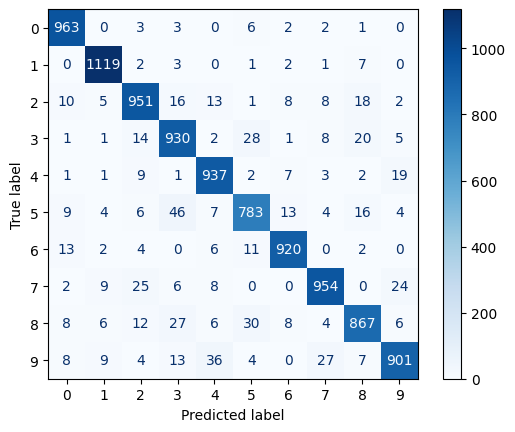
\includegraphics[width=0.8\textwidth]{figures/1-experiment/confusion_matrix_pca_svm_60000.png}
%     \caption{Confusion matrix for PCA with 60000 samples.}
%     \label{fig:confusion-matrix-pca-60000}
% \end{figure}
Table \ref{tab:classification-report-pca_svm_60000} shows the accuracy for \gls{svm} with \gls{pca} as dimensionality reduction with 60000 samples. The accuracy is 93.25\% for 60000 samples, and it takes 97 seconds to train the model, which is 1 minute and 37 seconds. The \gls{svm} model is best at recognizing zeros and ones in pictures, as the model has the f1-score in these classes, with scores of 96.5\% and 97.7\%. The model has some trouble recognizing fives, eights, and threes, as these are the lowest scoring in the f1-score for all the classes, with five being 89.1\%, eight being 90.6\%, and three being 90.5\%. \gls{svm} using \gls{pca} as the dimensionality reduction method has an average f1-score of 93.14\%.

\subsubsection{\gls{kpca} with 15000 samples}\label{subsubsec:experiment-1-results-kernel_pca-15000}
\begin{table}[htb!]
\centering
\caption{Classification report for kernel_pca_svm_15000}
\label{tab:classification-report-kernel_pca_svm_15000}
\begin{tabular}{lrrrr}
\toprule
 & precision & recall & f1-score & support \\
\midrule
0 & 0.943137 & 0.981633 & 0.962000 & 980.000000 \\
1 & 0.968858 & 0.986784 & 0.977739 & 1135.000000 \\
2 & 0.911005 & 0.922481 & 0.916707 & 1032.000000 \\
3 & 0.893175 & 0.894059 & 0.893617 & 1010.000000 \\
4 & 0.915842 & 0.941955 & 0.928715 & 982.000000 \\
5 & 0.881609 & 0.859865 & 0.870602 & 892.000000 \\
6 & 0.937824 & 0.944676 & 0.941238 & 958.000000 \\
7 & 0.929342 & 0.921206 & 0.925256 & 1028.000000 \\
8 & 0.927039 & 0.887064 & 0.906611 & 974.000000 \\
9 & 0.916667 & 0.883053 & 0.899546 & 1009.000000 \\
accuracy & 0.923600 & 0.923600 & 0.923600 & 0.923600 \\
macro avg & 0.922450 & 0.922278 & 0.922203 & 10000.000000 \\
weighted avg & 0.923360 & 0.923600 & 0.923321 & 10000.000000 \\
\bottomrule
\end{tabular}
\end{table}
 %92
\begin{figure}[htb!]
    \centering
    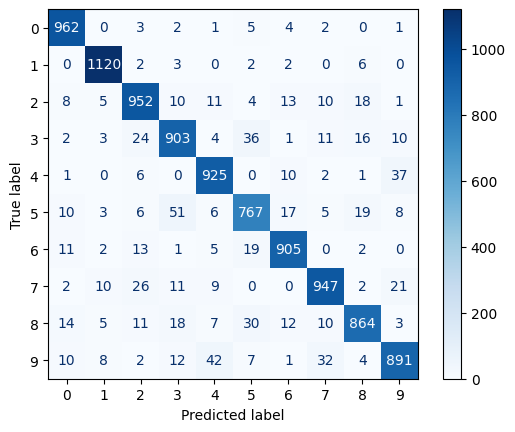
\includegraphics[width=0.8\textwidth]{figures/1-experiment/confusion_matrix_kernel_pca_svm_15000.png}
    \caption{Confusion matrix for kernel PCA with 15000 samples.}
    \label{fig:confusion-matrix-kpca-15000}
\end{figure}
Table \ref{tab:classification-report-kernel_pca_svm_15000} shows the accuracy for \gls{svm} with \gls{kpca} as dimensionality reduction with 15000 samples. The accuracy is 92.36\% for 15000 samples, and it takes 92 seconds to train the model, which is 1 minute and 32 seconds. \autoref{fig:confusion-matrix-kpca-15000} \gls{svm} model is best at recognizing zeros and ones in pictures, as the model has the f1-score in these classes, with scores of 96.2\% and 97.8\%. The model has trouble recognizing fives, nines, and threes, as these are the lowest scores in the f1-score for all the classes, with five being 87.1\%, nine being 90.0\%, and three being 89.4\%. \gls{svm} using \gls{kpca} as the dimensionality reduction method has an average f1-score of 92.22\%.

\subsubsection{\gls{isomap} with 15000 samples}\label{subsubsec:experiment-1-results-isomap-15000}
\begin{table}[htb!]
\centering
\begin{tabular}{lrrrr}
    \toprule
 & precision & recall & f1-score & support \\
\midrule
0 & 93.1507 & 97.1429 & 95.1049 & 980 \\
1 & 94.2953 & 99.0308 & 96.6051 & 1135 \\
2 & 92.1509 & 87.5969 & 89.8162 & 1032 \\
3 & 88.2579 & 90.7921 & 89.5071 & 1010 \\
4 & 91.5725 & 90.7332 & 91.1509 & 982 \\
5 & 87.7232 & 88.1166 & 87.9195 & 892 \\
6 & 95.1426 & 94.0501 & 94.5932 & 958 \\
7 & 88.5375 & 87.1595 & 87.8431 & 1028 \\
8 & 89.7297 & 85.2156 & 87.4144 & 974 \\
9 & 84.8963 & 85.2329 & 85.0643 & 1009 \\
accuracy & & & 90.6100 & 10000\\
macro avg & 90.5457 & 90.5071 & 90.5019 & 10000 \\
weighted avg & 90.5947 & 90.6100 & 90.5771 & 10000 \\
\bottomrule
\end{tabular}
\caption{Classification report for isomap\_svm\_15000}
\label{tab:classification-report-isomap_svm_15000}
\end{table}
 %165
\begin{figure}[htb!]
    \centering
    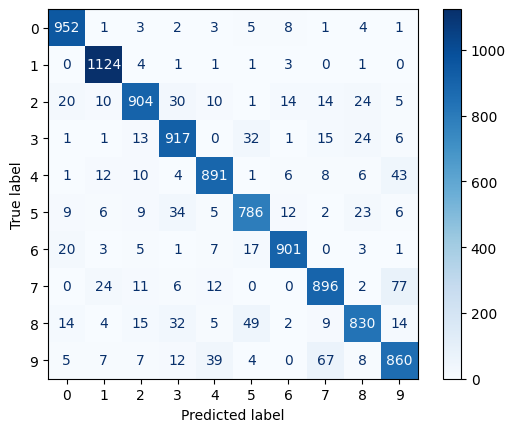
\includegraphics[width=0.8\textwidth]{figures/1-experiment/confusion_matrix_isomap_svm_15000.png}
    \caption{Confusion matrix for ISOMAP with 15000 samples.}
    \label{fig:confusion-matrix-isomap-15000}
\end{figure}
Table \ref{tab:classification-report-isomap_svm_15000} shows the accuracy for \gls{svm} with \gls{isomap} as dimensionality reduction with 15000 samples. The accuracy is 90.61\% for 15000 samples, and it takes 165 seconds to train the model, which is 2 minutes and 45 seconds. \autoref{fig:confusion-matrix-isomap-15000} \gls{svm} model is best at recognizing zeros and ones in pictures, as the model has the f1-score in these classes, with scores of 95.1\% and 96.6\%. The model has trouble recognizing sevens, eights, and nines, as these are the lowest scoring in the f1-score for all the classes, with seven being 87.8\%, eight being 87.4\%, and three being 85.1\%. \gls{svm} using \gls{isomap} as the dimensionality reduction method has an average f1-score of 90.50\%.

\subsection{Discussion experiment 1}\label{sec:discussion-experiment-1}
% discus the results to the problem statement
Comparing the results from experiment 1 is done in two comparisons; the first comparison is between the accuracy and time for the different dimensionality reduction methods. The second comparison is between the f1-scores for the different dimensionality reduction methods and what numbers the models are worst at recognizing. 

\subsubsection{Accuracy and time}\label{subsec:discussion-experiment-1-accuracy}
All experiments done is displayed in Table \ref{tab:discussion-experiment-1-accuracy}, it shows the accuracy for all the different models and the time taken.

\begin{table}
    \centering
    \begin{tabular}{lll}
        \hline
        Reduction method & Accuracy & Time \\
        \hline
        \gls{svm}-15 & 93.54\% & 37 seconds \\
        \gls{lda}-15 & 88.76\% & 7 seconds \\
        \gls{pca}-15 & 92.37\% & 10 seconds \\
        \gls{kpca}15 & 92.36\% & 92 seconds \\
        \gls{isomap}-15 & 90.61\% & 165 seconds \\
        \hline
        \gls{svm}-60 & 94.54\% & 378 seconds \\
        \gls{lda}-60 & 89.33\% & 58 seconds \\
        \gls{pca}-60 & 93.25\% & 97 seconds \\
        \hline
    \end{tabular}
    \caption{Accuracy and time for the different dimensionality reduction methods,  method-15 and method-60, means the method with 15 and 60 thousand samples.}
    \label{tab:discussion-experiment-1-accuracy}
    \end{table}
In \autoref{fig:discussion-experiment-1-plot} show the comparison between the methods with 15000 samples. The baseline \gls{svm}, on 15000 samples, has an accuracy of 93.54\%, and it takes 37 seconds to train the model. The baseline \gls{svm} can also be suitable to compare the other models, as it is an excellent model to hold as the baseline.

The accuracy increases by 1\% when using 45000 more samples, which is a slight difference. One thing to note is that it takes 37 seconds to train the model on 15000 samples and 378 seconds to train the model on 60000 samples. This means that the time it takes to train the model grows 921,62\% by using 45000 more examples of data. This is a big difference in time but a slight difference in accuracy.

\begin{figure}[htb!]
    \centering
    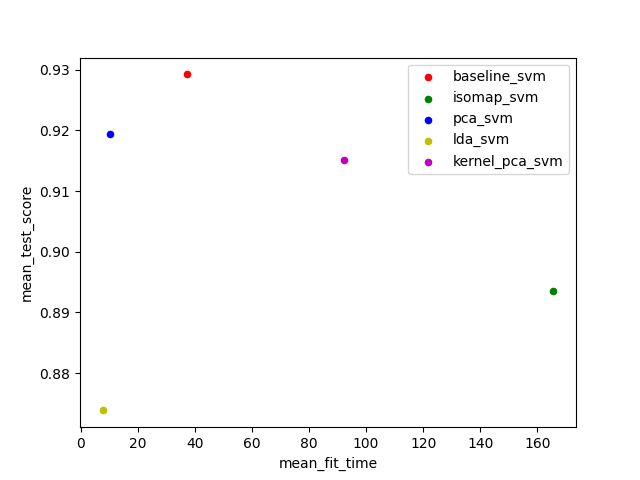
\includegraphics[width=0.8\textwidth]{figures/1-experiment/experiment1_plot.png}
    \caption{graph of time(in seconds) and accuracy(in percentage) for different dimensionality reduction methods}
    \label{fig:discussion-experiment-1-plot}
\end{figure}

When using \gls{lda} on 15000 samples, the accuracy falls to 88.76\%, but it only takes 7 seconds to train the model. \gls{lda} has a swift training time but low accuracy, but one thing to note, is that the maximum number of dimensions \gls{lda} can reduce to is 9 in this context. Therefore, the scores for \gls{lda} are worse than any dimensionality reduction method used. As the other methods use 49 dimensions to reduce the data, which is much higher than 9, it makes sense that the accuracy is higher than \gls{lda}. \gls{lda} only takes 7 seconds to train the model, so it is an excellent method to use if one wants a fast model with lower accuracy by comparing the other methods with more dimensions. 

When using 60000 samples, the accuracy is 89.33\%, and it takes 58 seconds to train the model. This means that the time it takes to train the model grows 728,57\% by using 45000 more examples of data. This is a big difference in time but a slight difference in accuracy; however, \gls{lda} is the fastest method, with lower accuracy than other methods. By using \gls{lda}, the model is faster but comes with the cost of lower accuracy.

When using \gls{pca} on 15000 samples, the accuracy is 92.37\%, and it takes 10 seconds to train the model, which is faster than the baseline \gls{svm} alone but still slower than \gls{lda} with the same amount of samples. When using 60000 samples, the accuracy is 93.25\%, and it takes 97 seconds to train the model. This means that the time it takes to train the model grows by 870\% by using 45000 more data samples. \gls{pca} has a lower accuracy than the baseline \gls{svm}. It is still faster than \gls{svm} alone but slower than \gls{lda}, making the model a good choice if one wants a faster model with slightly lower accuracy than the baseline \gls{svm}.

When using \gls{kpca} on 15000 samples, the accuracy is 92.36\%, and it takes 92 seconds to train the model. \gls{kpca} is slower than the baseline \gls{svm} and linear methods; this makes sense since nonlinear dimensionality methods can be heavier to compute. Nevertheless, \gls{kpca} scores the highest accuracy of all the dimensionality reduction methods used when using 15000 samples. If the computational cost is not an issue, \gls{kpca} is the best dimensionality reduction.

When using \gls{isomap} on 15000 samples, the accuracy is 90.61\%, and it takes 165 seconds to train the model. \gls{isomap} is slower than all the other dimensionality reduction methods and the baseline \gls{svm}. This makes sense since nonlinear dimensionality methods can be heavier to compute. However, \gls{isomap} scores the second lowest accuracy of all the dimensionality reduction methods used when using 15000 samples. So there are better dimensionality reduction methods than \gls{isomap} if one wants a fast model with high accuracy.

To conclude from this experiment, the baseline \gls{svm} is the best model to use if one wants a fast model with high accuracy. If one wants a faster model with lower accuracy, \gls{lda} is the best model to use. If one wants a model with high accuracy but slower than the baseline \gls{svm}, \gls{kpca} is the best model. If one wants a model with high accuracy but slower than the baseline \gls{svm}, \gls{isomap} is the best model. \gls{pca} is the best model if one wants a model with high accuracy and faster than the baseline SVM.

\subsubsection{F1-scores}\label{subsec:discussion-experiment-1-f1-score}
One thing to note is that the f1-score is the harmonic mean of precision and recall, which means that the f1-score is the average of the precision and recall. The f1-score is an excellent metric to use when the classes need to be balanced, as it is the average of precision and recall.
\begin{table}
    \centering
    \begin{tabular}{llrrr}
        \hline
        Reduction method & f1-score & worst score & 2. worst score & 3. worst score \\
        \hline
        \gls{svm}-15 & 93.43\% & 5 & 3 & 8 \\
        \gls{svm}-60 & 94.47\% & 5 & 8 & 3 \\
        \gls{lda}-15 & 88.59\% & 8 & 5 & 9 \\
        \gls{lda}-60 & 89.16\% & 8 & 5 & 3 \\
        \gls{pca}-15 & 92.25\% & 5 & 8 & 3 \\
        \gls{pca}-60 & 93.14\% & 5 & 3 & 8 \\
        \gls{kpca}-15 & 92.22\% & 5 & 3 & 9 \\
        \gls{isomap}-15 & 90.50\% & 9 & 8 & 7 \\
        \hline
    \end{tabular}
    \caption{F1-scores for the different dimensionality reduction methods.}
    \label{tab:discussion-experiment-1-f1-score}
    \end{table}
All experiments are displayed in Table \ref{tab:discussion-experiment-1-f1-score}, which shows the f1-score for the different models and the three worst classes for f1-scores.
In all experiments done, all of the models have a high f1-score, which means that the models are good at recognizing the numbers in the pictures. all models are best at recognizing zeros and ones in pictures. and good at recognizing four and sixes. When it comes to what the different models are bad at distinguishing, it is different for all. The most common number that the models are bad at recognizing is threes, fives, and eights, in a different order depending on the dimensionality reduction method used as these are the worst in \gls{svm} with both 15000 and 60000 samples, \gls{lda} with 60000 samples, \gls{pca} with 15000 samples and 60000 samples. \gls{isomap} is the only model that could be better at recognizing threes or fives, as it is terrible at sevens, eights, and nines. This can impact if one wants to use the model to find threes or fives; \gls{isomap} can be considered, as it is good at recognizing these numbers.

\gls{lda} with 15000 samples is interesting, as it needs to improve recognizing fives, eights, and nines. This is interesting as \gls{lda} with 60000 samples needs to improve recognizing threes, fives, and eights. This means \gls{lda} gets better at recognizing nines. This can be because more nines come into the dataset using 60000 samples, which makes \gls{lda} better at recognizing nines. 

In the occasions where there is more than one experiment done to the same method, the worst f1-scores for a class change, as seen in \gls{pca}, where at 15000 samples, the eights have the second worst f1-score, but at 60000 samples, the eights have the third worst f1-score. So the worst f1-scores for a class can change depending on the number of samples used.

To conclude this experiment, the models are good at recognizing the numbers in the pictures, but they are not perfect. The models are best at recognizing zeros and ones in pictures and recognizing four and sixes. When it comes to what the different models are bad at distinguishing, it is different for all. The most common number that the models are bad at recognizing is threes, fives, and eights, in a different order depending on the dimensionality reduction method used as these are the worst in \gls{svm} with both 15000 and 60000 samples, \gls{lda} with 60000 samples, \gls{pca} with 15000 samples and 60000 samples. \gls{isomap} is the only model that is not bad at recognizing threes or fives, as it is terrible at sevens, eights, and nines. This can have an impact if one wants to use the model to find threes or fives, \gls{isomap}P can be considered, as it is not bad at recognizing these numbers, but if one wants to use the model to find eights, then \gls{isomap} is not a good choice.

%intro
%presentation af de experimenter vi har valgt og hvorfor vi har valgt dem?
% experiment 1 exemple
%     detaljeret gennemgang af regler og evaluering
%     fremvisning af resultater
%     opsumering af resultater
%     diskussion af resultater og hvad der ellers var spændende evaluering af hvorfor det blev sådan.
%why this experiment was chosen
%look at f1-score and accuracy and time fitting the data
\section{Experiment 2}\label{sec:experiment-2}
This section will describe the second experiment of the project. The second experiment covers the necessary dimensions before reaching a threshold of 1\%, 5\%, and 10\% loss of accuracy. The experiment will only be done on 15.000 samples, instead of the entire dataset of 60.000 samples, due to issues regarding memory usage. The experiment will focus on when different dimensionality reduction methods drop in accuracy due to too few dimensions and compare them to each other to display the robustness of each of the methods.


\subsection{Rules and overview of the experiment}\label{subsec:experiment_2_rules}
This section will cover the rules of the second experiment and how the experiment results will be evaluated.

Every test in the second experiment is run on the same computer, pc-1. See \autoref{tab:pc1-specs} for the specific specs for the computer used in the experiment. It was first tried to run on another pc with less memory, but it was found that the nonlinear methods would take too long to run, and therefore it was run on pc-1.

For this experiment, the number of components will vary from around 2/5 to 50, and this range was chosen as it was believed to have a sufficient amount of components to show a general trend. For the nonlinear methods, 5 components, instead of 2, were chosen as the lowest amount, as the nonlinear methods gave errors when using fewer components than 5.

\gls{lda} is an exception, as the maximum number of components is the number of classes $-1$, which is 9 for the \gls{mnist} dataset, which means that the range of components for \gls{lda} will be from 2-9.

The values used to evaluate this experiment are \texttt{mean\_test\_score} based on \texttt{param\_pca\_\_n\_components} to evaluate the model's accuracy with the number of components used.

For each experiment, the data will be analyzed to see how many components can be removed before the accuracy drops below a certain threshold. For the experiment's sake, the thresholds will be based on the best accuracy score for each method. The thresholds will be a 1\% loss in accuracy, a 5\% loss in accuracy, and a 10\% loss in accuracy. If a method has the best accuracy score of 96\%, the thresholds will be 96 - 1\% = 95.05, 96 - 5\% = 91.20, and 96 - 10\% = 86.40. These thresholds were chosen as they are believed to be a good balance between the number of components that can be removed and the amount of accuracy lost, which could be acceptable for some use cases.


\subsection{Results}\label{subsec:experiment_2_results}
This section will cover the results gathered from running the second experiment. Each of the dimensionality reduction methods will be presented using scatter plots. The scatter plots will show the number of components used along the x-axis and the model's accuracy along the y-axis. Each component has multiple dots, so the accuracy varies slightly depending on the hyperparameters used, but the general trend is the same. The results will then be compared and evaluated based on the experiment's rules.

The main focus of the evaluation will be on when the accuracy starts to drop noticeably and how many components are needed to have good accuracy still. The scatter plots are used to represent the results visually, and the specific values of the accuracy will also be discussed. These values are taken from the csv files generated from running the second experiment.

\subsubsection{\gls{pca}}\label{subsubsec:experiment_2_pca}
\gls{pca} is a linear dimensionality reduction method; the scatter plot representing this method can be seen in \autoref{fig:experiment_2_pca_svm}.

As one would expect, the model's accuracy increases as the number of components increases. However, around 20 components, the accuracy starts to drop, the accuracy especially has a noticeable drop between 10 and 20 components, and the accuracy has a drastic drop for each component removed below ten components. This is expected as the lower the number of components the model has to work with; the more information is lost.

\begin{figure}[htb!]
    \centering
    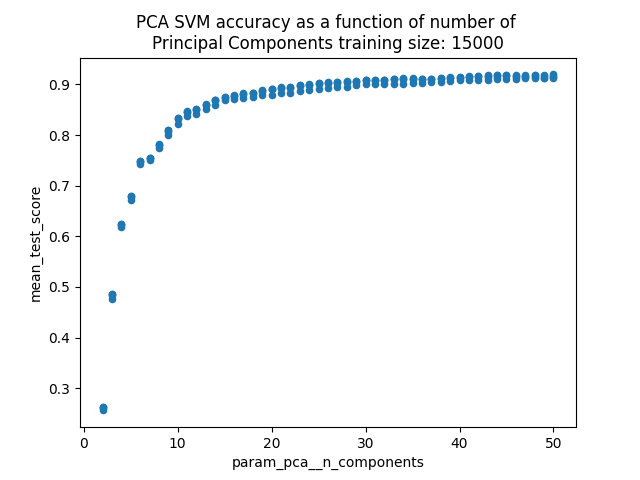
\includegraphics[width=0.8\textwidth]{figures/experiment_two/pca_svm_15000.png}
    \caption{Accuracy of the SVM model with \gls{pca} as dimensionality reduction method, with the number of components used.}
    \label{fig:experiment_2_pca_svm}
\end{figure}

For \gls{pca}, the highest accuracy value is 91.99\% with 50 components and the value 0.01 for the C hyperparameter in \gls{svm}. The thresholds for \gls{pca} are: 91.99 - 1\% = 91.07, 91.99 - 5\% = 87.39, and 91.99 - 10\% = 82.79. The results of the experiment for \gls{pca} will be compared to these thresholds.

By sorting the data by \texttt{mean\_test\_score} and going through the values, given the best-case scenario with the best hyperparameters found. The first value that drops below the threshold of 91.07\% is with an accuracy of 90.57\% at 29 components, which means that the model's accuracy only increases by 1\% with the last 21 components, which is close to half the total amount of components.
The next threshold of 87.39\% accuracy is found at 86.86\% with 14 components. By removing an additional seven components, the accuracy dropped from a 1\% loss to a 5\% loss.
The final threshold of 82.79\% accuracy is found at 80.70\% with nine components. By removing only five components, the accuracy dropped from a 5\% loss to a 10\% loss.

\subsubsection{Linear discriminant analysis}\label{subsubsec:experiment_2_lda}
The scatter plot representing \gls{lda} method can be seen in \autoref{fig:experiment_2_lda_svm}. \gls{lda} reduces the dimension to the number of classes $-1$, which is why the total number of components used is nine since \gls{mnist} has ten different numbers. The general trend is still valid for discussion in the second experiment.


\begin{figure}[htb!]
    \centering
    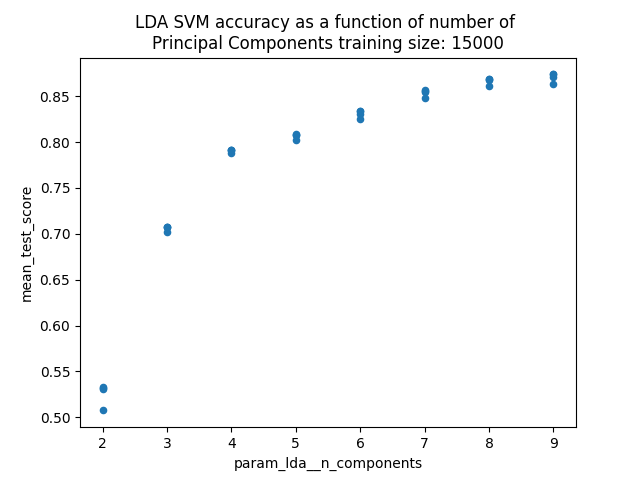
\includegraphics[width=0.8\textwidth]{figures/experiment_two/lda_svm_15000.png}
    \caption{Accuracy of the SVM model with \gls{lda} as dimensionality reduction method, with the number of components used.}
    \label{fig:experiment_2_lda_svm}
\end{figure}

For \gls{lda}, the highest accuracy score is at 87.38\% with nine components and the value 0.1 for the C hyperparameter in \gls{svm}. The thresholds for \gls{lda} are: 87.38 - 1\% = 86.50, 87.38 - 5\% = 83.01, and 87.38 - 10\% = 78.64. The experiment's results for \gls{lda} will be compared to these thresholds.

Repeating the method of looking through the data gathered, the first value that drops below the first threshold  of 86.50\%, with the 0.1 hyperparameter, is at 85.61\% with seven components.

The next threshold of 83.01\% accuracy is found at 80.83\% with five components. By removing two components, the accuracy dropped from a 1\% loss to a 5\% loss, which is not many components when compared to \gls{pca}, but for \gls{lda} that only has nine total components, a large percentage of the components can be removed with only a 5\% accuracy loss.

The final threshold of 78.64\% accuracy is found at 70.75\% with only three components. They are showing a significant drop from the threshold since the first few components impact the accuracy score significantly, and the closest value to the threshold is ~8\% away.


\subsubsection{\gls{kpca}}\label{subsubsec:experiment_2_kpca}
\gls{kpca} is a nonlinear dimensionality reduction method, and the scatter plot representing this method can be seen in \autoref{fig:experiment_2_kpca_svm}.

\begin{figure}[htb!]
    \centering
    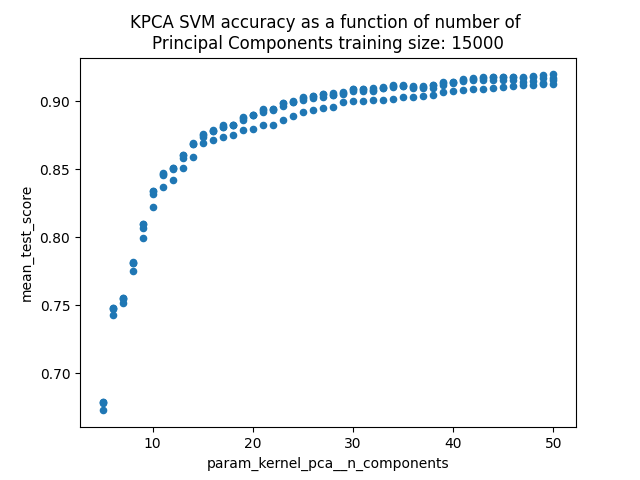
\includegraphics[width=0.8\textwidth]{figures/experiment_two/kpca_svm_15000.png}
    \caption{Accuracy of the SVM model with \gls{kpca} as dimensionality reduction method, with the number of components used.}
    \label{fig:experiment_2_kpca_svm}
\end{figure}

\autoref{fig:experiment_2_kpca_svm} is very similar to the other methods, and almost identical with \autoref{fig:experiment_2_pca_svm}, the only difference is that \gls{kpca} uses at minimum 5 components, where \gls{pca} uses at the lowest 2 components.

\gls{kpca} has a top accuracy score of 91.99\% with the value 0.01 for the C hyperparameter in \gls{svm}, meaning that the thresholds for \gls{kpca} are: 91.99 - 1\% = 91.07, 91.9 - 5\% = 87.39, and 91.9 - 10\% = 82.79. The experiment's results for \gls{kpca} will be compared to these thresholds.

Similar to linear methods, the data is sorted by its accuracy score to find the first value where the accuracy drops below a threshold, that uses the same hyperparameter. The first threshold of 91.07\% accuracy is found at 91.04\% with 34 components. The next threshold of 87.39\% accuracy is found at 86.86\% with 14 components. The final threshold of 82.79\% accuracy is found at 80.70\% with nine components.


\subsubsection{\gls{isomap}}\label{subsubsec:experiment_2_isomap}
\gls{isomap} is the final method of the second experiment, which is nonlinear, and the scatter plot representing this method can be seen in \autoref{fig:experiment_2_isomap_svm}.

\begin{figure}[htb!]
    \centering
    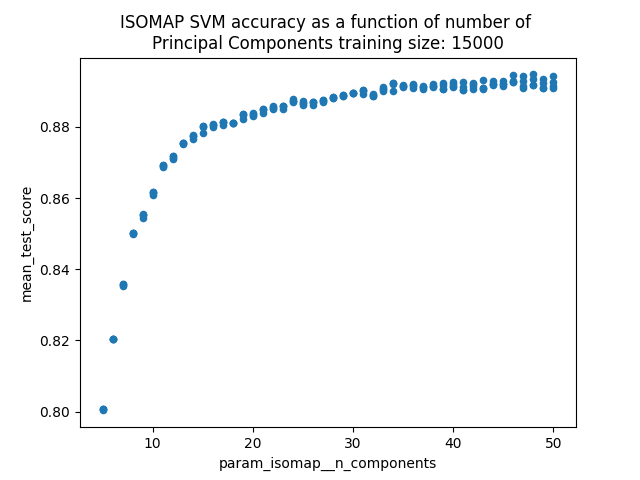
\includegraphics[width=0.8\textwidth]{figures/experiment_two/isomap_rerun_svm_15000.png}
    \caption{Accuracy of the SVM model with \gls{isomap} as dimensionality reduction method, with the number of components used.}
    \label{fig:experiment_2_isomap_svm}
\end{figure}

\autoref{fig:experiment_2_isomap_svm} is similar to the other methods as the accuracy drops drastically as the number of components decreases, but interestingly even the lowest accuracy for \gls{isomap} is still relatively high. The span from best to worst accuracy is much smaller than the other methods. The highest accuracy score for \gls{isomap} is 89.4\% with 48 components and the value 0.001 for the C hyperparameter in \gls{svm}, and the lowest accuracy score is 80\% with five components. The best and worst accuracy scores are closer together than the other methods, with only a ~9\% difference.

isomap has a top accuracy score of 89.47\%, with 48 components, and the value 0.001 for the C hyperparameter in \gls{svm}. meaning that the thresholds for \gls{isomap} are: 89.47 - 1\% = 88.57, 89.47 - 5\% = 84.99, and 89.47 - 10\% = 80.52.

The first threshold of 88.57\% accuracy is found at 88.49\% with 22 components, the next threshold of 84.99\% accuracy is found at 83.54\% with seven components, and the final threshold of 79.4\% accuracy is not found in the data, as the lowest accuracy score is 80.8\% with five components. To still be able to compare the results of \gls{isomap}  with the other methods, the lowest accuracy score will be used as the threshold, but it should be made clear that the actual threshold is not found in the data.


\subsection{Discussion of experiment 2}\label{subsec:experiment_2_discussion}
This section will discuss the results of the second experiment and compare the results of the different methods, first by discussing the results of the linear methods, then the nonlinear methods, and finally, comparing the results of all methods.

For each section, a table will display the different percentages of components remaining before the accuracy drops below a threshold. The table will also show the number of remaining components to show the difference between the methods.


\subsubsection{Linear methods}
By comparing the two linear methods used for the second experiment, it is essential to know that the number of components is very different between \gls{pca} \gls{lda}, which means that an exact comparison between the two methods is not always clear. Instead of using the number of components as a comparison, the percentage of remaining components will be used to try and make a fair comparison. A table showing the differences between the two methods can be seen in \autoref{tab:experiment_2_linear_methods_comparison}.

\begin{table}[htb!]
    \centering
    \begin{tabular}{cp{0.15\textwidth}p{0.15\textwidth}}
        \toprule
        \textbf{Thresholds} & \textbf{PCA \% 50} & \textbf{LDA \% 9} \\
        \midrule
        1\%                 & 58\% (29)          & 77.7\% (7)        \\
        5\%                 & 28\% (14)          & 55.5\% (5)        \\
        10\%                & 18\% (9)           & 33.3\% (3)        \\
        \bottomrule
    \end{tabular}
    \caption{Percentage of the components remaining after the threshold is reached, with the corresponding number of components in paratheses.}
    \label{tab:experiment_2_linear_methods_comparison}
\end{table}

\autoref{tab:experiment_2_linear_methods_comparison} shows, for each linear method, the amount of components left after each of the thresholds is reached. So for \gls{pca}, 58\% of the total number of components remain before reaching the first threshold of 1\%, whereas, for \gls{lda}, there is 77.7\%.

From \autoref{tab:experiment_2_linear_methods_comparison}, it can be seen that before reaching the first threshold of losing 1\% accuracy, \gls{pca} can cut off 42\% of its components, while \gls{lda} can can only cut off 22.3\%.

By comparing the two linear methods, it can be concluded that \gls{lda} is more prone to losing accuracy when removing components than \gls{pca}. The accuracy loss is likely because \gls{lda} has so few components to work with in the first place. It could be argued that the results are not entirely fair since \gls{pca} has so many more components, but scaling the values with percentage should show a general trend.


\subsubsection{nonlinear methods}
Unlike the linear methods, the nonlinear methods have a similar number of components, which should give a more fair comparison. A table showing when the respective thresholds were reached for each of the nonlinear methods can be seen in \autoref{tab:experiment_2_non_linear_methods_comparison}.

\begin{table}[htb!]
    \centering
    \begin{tabular}{cp{0.20\textwidth}p{0.20\textwidth}}
        \toprule
        \textbf{Thresholds} & \textbf{KPCA \% 50} & \textbf{ISOMAP \% 50} \\
        \midrule
        1\%                 & 68\% (34)           & 40\% (22)             \\
        5\%                 & 28\% (14)           & 14\% (7)              \\
        10\%                & 18\% (9)            & 1\% (5)*              \\
        \bottomrule
    \end{tabular}
    \caption{Percentage of the components remaining after the threshold is reached, with the corresponding number of components in paratheses.}
    \label{tab:experiment_2_non_linear_methods_comparison}
\end{table}

Figure 1 shows that \gls{kpca} and \gls{isomap} can afford to cut off a significant amount of components before reaching the first threshold of 1\%. \gls{kpca} can cut off 42\% of its components, while \gls{isomap} can cut off 60\% of its components. Another interesting note is that \gls{isomap} never reaches the 10\% accuracy loss threshold, and the closest accuracy score is used instead. Although it is not entirely accurate, the percentage from the actual threshold is <1\%, so for the sake of the comparison, it will be assumed that the threshold was reached.

Generally, it can be concluded that both \gls{kpca} and \gls{isomap} can afford to cut off a significant amount of components before losing accuracy. It is interesting to note that \gls{isomap} can cut off more components than \gls{kpca} before losing accuracy. However, \gls{kpca} reaches a higher accuracy score than \gls{isomap} but also reaches a lower accuracy score than \gls{isomap}, which means that \gls{isomap} could be considered more consistent than kpca, as the span of accuracy score for \gls{isomap} is smaller.


\subsubsection{Comparison of methods}
Now that the linear and nonlinear methods have been compared, it is time to compare the methods to each other. The results can be seen in \autoref{tab:experiment_2_methods_comparison}.


\begin{table}[htb!]
    \centering
    \begin{tabular}{cp{0.15\textwidth}p{0.15\textwidth}p{0.15\textwidth}p{0.20\textwidth}}
        \toprule
        \textbf{Thresholds} & \textbf{PCA \% 50} & \textbf{LDA \% 9} & \textbf{KPCA \% 50} & \textbf{ISOMAP \% 50} \\ \midrule
        1\%                 & 58\% (29)          & 77.7\% (7)        & 58\% (34)           & 40\% (22)             \\
        5\%                 & 28\% (14)          & 55.5\% (5)        & 28\% (14)           & 14\% (7)              \\
        10\%                & 18\% (9)           & 33.3\% (3)        & 18\% (9)            & 1\% (5)*              \\
        \bottomrule
    \end{tabular}
    \caption{Percentage of the components remaining after the threshold is reached, with the corresponding number of components in paratheses.}
    \label{tab:experiment_2_methods_comparison}
\end{table}

The first noticeable thing is that \gls{pca} and \gls{kpca} are similar in the number of components they can cut off before losing accuracy enough to reach the thresholds. The highest accuracy score is the same between the two methods, but the lowest accuracy score is lower for PCA, this lower accuracy score is likely due to the range of components \gls{pca} has.  The lower the percentage in \autoref{tab:experiment_2_methods_comparison}, the more components can be cut off without losing accuracy. So from this, it can be concluded that \gls{lda} is the method that has the most drastic accuracy loss when cutting off components. This is likely because \gls{lda} has so few components to work in the first place, and therefore it is more sensitive to the removal of components. \gls{isomap} is the method that has the most negligible accuracy loss when cutting off components. Additionally, \gls{isomap}'s worst accuracy score is better than any other method, but its best accuracy score is also the lowest.

From the second experiment, it can be concluded that \gls{isomap} is the method that can cut off most components before losing accuracy. However, each method has its strengths and weaknesses, and it is essential to consider the context of the problem when choosing a method.


% intro
% presentation af de experimenter vi har valgt og hvorfor vi har valgt dem?
% experiment 1 exemple
%     detaljeret gennemgang af regler og evaluering
%     fremvisning af resultater
%     opsumering af resultater
%     diskussion af resultater og hvad der ellers var spændende evaluering af hvorfor det blev sådan.

%logarithmic regression
%Bar chart
\section{Experiment 3}
This experiment is targetted towards \gls{pca} and \gls{kpca}. The goal is to compare the performance of \gls{pca} and \gls{kpca}, because these methods are similar, with the exception that \gls{kpca} implements a kernel. Beause of the similarity of the methods, comparison will be more focused on the impact the different kernels can have on the model, namely what numbers does the machine learning model confuse given the different kernels.


As explained in the Chapter Theory, KPCA can have kernels, which will project the data into a higher dimensional feature space, where a hyperplane can be constructed, and perform PCA on it. KPCA does not require the transformation of the inputs into the feature space with the kernel function, but can use the kernels so as to get the dot product of the pair-wise input points~\cite{kpca-book}.


The kernels are a measure of similarity between the points~\cite{scikit-learn}, which means that points that are close to each other have higher similarity score, which is computed with the kernel function. The kernels chosen for the experiment are the \gls{rbf} and sigmoid kernels. The sigmoid kernel \textcquote{scikit-learn}{computes the sigmoid kernel between two vectors}, which outputs a value between -1 and 1 for the two given input vectors. The \gls{rbf} kernel \textcquote{scikit-learn}{computes the radial basis function kernel between two vectors}, which outputs a value between 0 and 1.


\subsection{Rules}
This experiment will not use gridsearch. The input of the data samples will be 15000 for both of the methods, because of hardware limitations. The amount of components used for the methods will be the ones that were used in experiment one, namely 49 components. The evaluation will be based on the confusion matrices, and eventually also for the score of the methods. The kernels used will be \gls{rbf} and sigmoid.


\subsection{Results}
Figure \ref{fig:confusion-matrix-pca-svm} shows the results for \gls{pca}.
Figure~\ref{fig:confusion-matrix-kernel-pca-svm-sigmoid} shows the results for \gls{kpca} with sigmoid kernel.
Figure~\ref{fig:confusion-matrix-kernel-pca-svm-rbf} shows the results for \gls{kpca} with rbf kernel.


\begin{figure}[htb!]
    \centering
    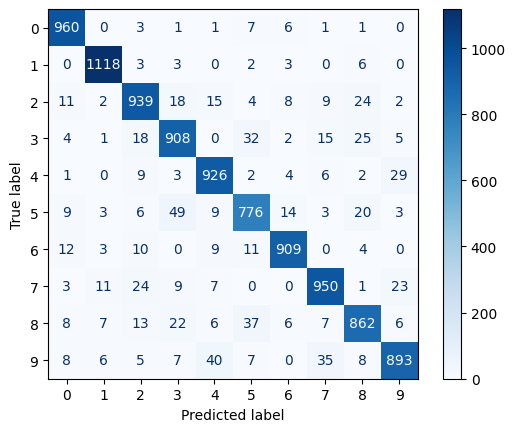
\includegraphics[width=0.5\textwidth]{../src/results/experiment_three/confusion_matrix_pca_svm.png}
    \caption{Confusion matrix for PCA}
    \label{fig:confusion-matrix-pca-svm}
\end{figure}





\begin{figure}
    \centering
    \subfloat[\centering Confusion matrix for kPCA Sigmoid]{\label{fig:confusion-matrix-kernel-pca-svm-sigmoid}{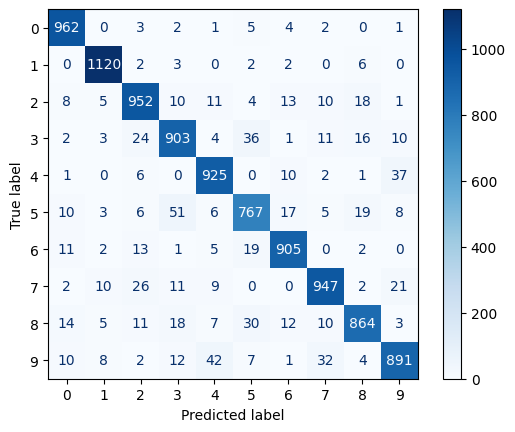
\includegraphics[width=0.45\textwidth]{../src/results/experiment_three/confusion_matrix_kernel_pca_svm_sigmoid.png} }}
    \qquad
    \subfloat[\centering Confusion matrix for kPCA RBF]{\label{fig:confusion-matrix-kernel-pca-svm-rbf}{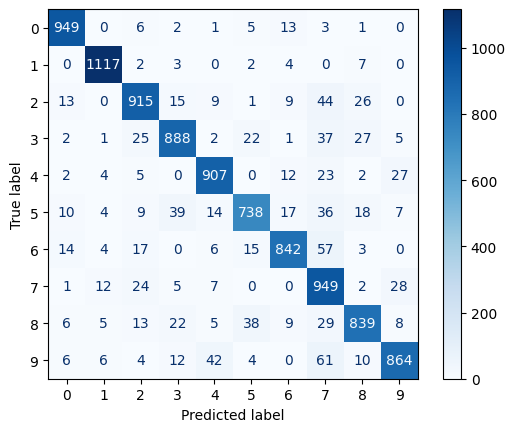
\includegraphics[width=0.45\textwidth]{../src/results/experiment_three/kernel_pca_rbf_kernel_49.png} }}%
    \caption{both kPCA kernels confusion matrices}
    \label{fig:kpca-kernels}
\end{figure}






\subsection{Results}
A slight improvement over the number 0 has been seen in \gls{kpca-s} in that it mapped 11 numbers better than \gls{pca}, and the same can be said for the number 2.

Both methods acquired the same amount of correct predictions for the numbers 3 and 4.

A slight difference appears in the number 5, where \gls{pca} has 780 correct predictions, and \gls{kpca-s} got 767, which is worse than \gls{pca}. The reason for that is because it confused it with the numbers 3 and 6.


A slight improvement in \gls{kpca-s} is seen at the number 6, where it got five numbers more than \gls{pca}. Such a low number is not worth considering, however.

It can be seen that sigmoid confuses the number 7 with the number 9 more often than \gls{pca} normally would, which worsens \gls{kpca-s}' ability to predict the number 7 correctly.

The notable impressions regarding the differences between \gls{pca} and \gls{kpca-s} are: \gls{kpca-s} improved by about ten numbers at the numbers 0 and 2, became worse at the number 5, became worse at the number 7, and shined the most at the number 8. The most interesting cases are the numbers 0,2, 5, and 8.


The RBF kernel has confused more number 2's than any other method presented in this experiment. As opposed to \gls{pca} and \gls{kpca-s}, \gls{kpca-r} confused it 33 times more with the number 7 and around ten times more with the number 8. The same pattern can be seen at the number 3, where it was again confused with numbers 7 and 8.


\gls{kpca-r} has confused the number 4 mainly with the numbers 7 and 9, and \gls{kpca-s} has only confused it with the number 9. Concerning the number 4, \gls{kpca-s} is the only method that has confused it the most with the number 9.


\gls{kpca-r} mainly confuses the number 5 with the numbers 3 and 7, whereas \gls{kpca-s} does it with the numbers 3, 6, and 8, and the same can be said about \gls{pca}.

The number 6 reveals a potentially interesting finding: \gls{kpca-r} is the only method that managed to confuse the number 6 with the number 7, as opposed to the other methods, which did not confuse it with the number 7.

The only place where \gls{kpca-r} outshines \gls{kpca-s} is at the number 7, where \gls{kpca-r} confuses with two numbers less than \gls{kpca-s}. Such a finding, however, is not of major importance because \gls{kpca-r} underperforms most of the time. 

\subsubsection{Summary of the differences between the methods}
From the results presented so far about the differences between the kernels it can be seen that all the methods often confuse the number 2 with 8; 3 with 2,5,8 and to a certain degree(PCA and much worse with \gls{kpca-r}), 7. The methods also confuse the number 4 with 9; 5 with 3,6, and 8 (\gls{kpca-r} also does it with 7). The number 6 gets confused with the number 0,2,5 (\gls{kpca-r} also does it with 7).
The number 7 gets confused with the number 2,3 and 9. \gls{kpca-r} is the only one that did not confuse the number 3 as much as the other methods.

At number 8, the methods have confused 0 (except for \gls{kpca-r}),2,3 and 5. \gls{kpca-r} confused it again with the number 7, but it is the only one that managed to map the number 0 less than the other methods. Lastly the number 9 got confused with the numbers the most with the numbers 4 and 7. It can be further noted that \gls{kpca-r} is the worst at confusing various numbers with the number 7.


From the overview provided regarding the difference in numbers, a percentage would be more preferable, more specifically, a percentage of the errors made in the numbers 0-9. Table \ref{tab:error-percentage-pca-kpca-s-kpca-r} shows the difference in percentages of errors made by the methods for each number.

\begin{table}[htb!]
    \centering
    \begin{tabular}{lrrrr}
        \toprule
          & pca    & kpca-s & kpca-r \\
        \midrule
        0 & 2.959  & 1.836  & 3.163  \\
        1 & 1.585  & 1.321  & 1.585  \\
        2 & 8.817  & 7.751  & 11.337 \\
        3 & 10.594 & 10.594 & 12.079 \\
        4 & 5.702  & 5.804  & 7.637  \\
        5 & 12.556 & 14.013 & 17.264 \\
        6 & 6.054  & 5.532  & 12.108 \\
        7 & 7.101  & 7.879  & 7.684  \\
        8 & 13.552 & 11.293 & 13.860 \\
        9 & 11.992 & 11.694 & 14.370 \\
        \bottomrule
    \end{tabular}
    \caption{Error percentage for each number for the methods}
    \label{tab:error-percentage-pca-kpca-s-kpca-r}
\end{table}

Another finding which could be explored is the difference in the number of errors made by the methods for each number. Table \ref{tab:error-percentage-pca-kpca-s-kpca-r} shows the difference in the number of errors made by the methods for each number.

Yet another finding that could be explored is to research why \gls{kpca-r} is the only method that confuses many numbers with the number 7.
%\subsection{Discussion of results}


\section{Experiment 4}\label{sec:experiment-4}

In this experiment, a machine learning pipeline is used to explore the effects of different sizes of samples on the performance of linear and non-linear dimensionality reduction methods. The \gls{mnist} data set is used as the source of data, and a range of sample sizes are selected, starting with 200 and ending with 5000. The pipeline uses \gls{svm} as the model and applies four different dimensionality reduction techniques: \gls{pca}, \gls{lda}, \gls{kpca}, and \gls{isomap}.

The performance of the pipeline is evaluated using three metrics: accuracy, f1-score, and time. The results of the experiment are analyzed to compare the performance of the different dimensionality reduction methods under varying sample sizes and to explore the differences between linear and non-linear approaches.

Overall, the results of this experiment provide insight into the factors that can influence the effectiveness of dimensionality reduction in machine learning and can inform the choice of dimensionality reduction method in real-world scenarios. Furthermore, the findings can contribute to the broader understanding of the role of sample size in the performance of machine learning models and dimensionality reduction.

\subsection{Parameters and evaluation}
In this experiment the same general hyper parameter tuning as in experiment 1 will be used on datasamples from \gls{mnist} of the size 200, 300, 400, 500, 600, 700, 800, 900, 1000, 2000, 3000, 4000, 5000. It will be evaluated based on f1, accuracy and how much time it uses.




\subsection{Results}\label{subsec:experiment_4_results}
In this section, we present the results of the fourth experiment, which compare the performance of different dimensionality reduction methods on a classification task. We show the results for different sample sizes using confusion matrices and tables, as well as scatter plots to visualize the relationship between sample size, accuracy, and time taken. We evaluate the results based on the rules of the experiment, focusing on accuracy, F1 score, time taken, and the size of the sample required to achieve good accuracy. We also discuss the specific values of accuracy obtained from the csv files generated by the experiment. The scatter plots provide a visual representation of the results and make it easy to see when accuracy and time start to improve. generally each method and the base case will show the results of the samples 200, 1000, 5000.

\subsubsection{\gls{svm} Model}\label{subsubsec:experiment_4_no_dimmensionality_reduction}

\begin{table}[htb!]
\centering
\begin{tabular}{lrrrr}
    \toprule
 & precision & recall & f1-score & support \\
 \midrule
 0 & 83.0224 & 90.8163 & 86.7446 & 980 \\
 1 & 78.2424 & 97.2687 & 86.7243 & 1135 \\
 2 & 67.8335 & 69.4767 & 68.6453 & 1032 \\
 3 & 73.6059 & 78.4158 & 75.9348 & 1010 \\
 4 & 70.7377 & 87.8819 & 78.3833 & 982 \\
 5 & 71.6243 & 41.0314 & 52.1739 & 892 \\
 6 & 91.3043 & 63.5699 & 74.9538 & 958 \\
 7 & 78.3178 & 81.5175 & 79.8856 & 1028 \\
 8 & 73.1092 & 71.4579 & 72.2741 & 974 \\
 9 & 71.7842 & 68.5828 & 70.1470 & 1009 \\
 accuracy & & & 756700 & 10000 \\
 macro avg & 75.9582 & 75.0019 & 74.5867 & 10000 \\
 weighted avg & 75.9485 & 75.6700 & 74.9591 & 10000 \\
 \bottomrule
\end{tabular}
\caption{Classification report for baseline\_svm\_200}
\label{tab:classification-report-baseline_svm_200}
\end{table}

\begin{table}[htb!]
\centering
\caption{Classification report for baseline_svm_1000}
\label{tab:classification-report-baseline_svm_1000}
\begin{tabular}{lrrrr}
\toprule
 & precision & recall & f1-score & support \\
\midrule
0 & 0.925998 & 0.970408 & 0.947683 & 980.000000 \\
1 & 0.921667 & 0.974449 & 0.947323 & 1135.000000 \\
2 & 0.865842 & 0.881783 & 0.873740 & 1032.000000 \\
3 & 0.877095 & 0.777228 & 0.824147 & 1010.000000 \\
4 & 0.867005 & 0.869654 & 0.868327 & 982.000000 \\
5 & 0.785340 & 0.840807 & 0.812128 & 892.000000 \\
6 & 0.914621 & 0.894572 & 0.904485 & 958.000000 \\
7 & 0.860927 & 0.885214 & 0.872902 & 1028.000000 \\
8 & 0.864350 & 0.791581 & 0.826367 & 974.000000 \\
9 & 0.822178 & 0.815659 & 0.818905 & 1009.000000 \\
accuracy & 0.871700 & 0.871700 & 0.871700 & 0.871700 \\
macro avg & 0.870502 & 0.870136 & 0.869601 & 10000.000000 \\
weighted avg & 0.871760 & 0.871700 & 0.871014 & 10000.000000 \\
\bottomrule
\end{tabular}
\end{table}

\begin{table}[htb!]
\centering
\begin{tabular}{lrrrr}
    \toprule
    & precision & recall & f1-score & support \\
    \midrule
    0 & 0.955224 & 0.979592 & 0.967254 & 980.000000 \\
    1 & 0.953072 & 0.984141 & 0.968357 & 1135.000000 \\
    2 & 0.909980 & 0.901163 & 0.905550 & 1032.000000 \\
    3 & 0.890279 & 0.915842 & 0.902879 & 1010.000000 \\
    4 & 0.904854 & 0.949084 & 0.926441 & 982.000000 \\
5 & 0.901278 & 0.869955 & 0.885339 & 892.000000 \\
6 & 0.952128 & 0.934238 & 0.943098 & 958.000000 \\
7 & 0.925123 & 0.913424 & 0.919236 & 1028.000000 \\
8 & 0.904555 & 0.856263 & 0.879747 & 974.000000 \\
9 & 0.902414 & 0.888999 & 0.895657 & 1009.000000 \\
accuracy & 0.920500 & 0.920500 & 0.920500 & 0.920500 \\
macro avg & 0.919891 & 0.919270 & 0.919356 & 10000.000000 \\
weighted avg & 0.920338 & 0.920500 & 0.920197 & 10000.000000 \\
\bottomrule
\end{tabular}
\caption{Classification report for baseline\_svm\_5000}
\label{tab:classification-report-baseline_svm_5000}
\end{table}


The first part of the experiment involved running a machine learning pipeline without applying any dimensionality reduction. The pipeline used a \gls{svm} model and was trained on the \gls{mnist} data set. The sample size for this part of the experiment was 100.

The results of this experiment are shown in \ref{tab:classification-report-baseline_svm_200}. The table shows the precision, recall, and f1-score for each of the ten classes in the data set, as well as the overall accuracy of the model. The table also shows the macro average and weighted average scores.

Overall, the results show that the \gls{svm} model achieved an accuracy of approximately 67\%. This indicates that the model performed relatively well but still had some errors in its predictions. The precision and recall scores for each class varied, with some classes having higher scores than others. For example, the model had a precision of approximately 87\% for class 0 but only a precision of approximately 45\% for class 9. 

These results provide a baseline for comparison with the results of the other parts of the experiment, in which different dimensionality reduction methods were applied. The results of this initial experiment will be used to evaluate the effectiveness of the different dimensionality reduction methods in improving the performance of the \gls{svm} model.

The second part of the base case involved using a sample size of 1000; it can be seen in \ref{tab:classification-report-baseline_svm_1000}. Compared to the results of the first part of the experiment, the accuracy of the \gls{svm} model improved significantly, achieving an accuracy of approximately 87\%. This indicates that using a larger sample size improved the performance of the model. The precision and recall scores for each class also improved, with most classes having higher scores than in the first part of the experiment.

The next sample of size 5000 can be seen in \ref{tab:classification-report-baseline_svm_5000}.
Comparing \ref{tab:classification-report-baseline_svm_5000} and \ref{tab:classification-report-baseline_svm_5000}, it is clear that the \gls{svm} model achieved higher accuracy and precision when trained on a larger sample size. For example, the accuracy of the model increased from 87\% for the 1000-sample data set to 92\% for the 5000-sample data set. Similarly, the precision of the model increased for most of the classes, with the largest increase being seen for class 5, where the precision increased from 78\% to 90\%.

Additionally, the f1-score, which is a measure of the balance between precision and recall, also improved for most classes when using a larger sample size. This suggests that the model was able to make more accurate predictions and avoid false positives and false negatives more effectively when trained on a larger data set.


\subsubsection{\gls{pca}}\label{subsubsec:experiment_4_pca}

The second part of the experiment involved running a machine learning pipeline applying \gls{pca} as a dimensionality reduction method. The sample sizes for this part of the experiment were 200, 1000, and 5000.

\begin{table}[htb!]
    \centering
    \begin{tabular}{lrrrr}
        \toprule
        & precision & recall & f1-score & support \\
        \midrule
        0 & 0.838207 & 0.877551 & 0.857428 & 980.000000 \\
        1 & 0.770701 & 0.959471 & 0.854788 & 1135.000000 \\
        2 & 0.675052 & 0.624031 & 0.648540 & 1032.000000 \\
        3 & 0.744227 & 0.829703 & 0.784644 & 1010.000000 \\
        4 & 0.692244 & 0.845214 & 0.761119 & 982.000000 \\
        5 & 0.747492 & 0.501121 & 0.600000 & 892.000000 \\
        6 & 0.931649 & 0.654489 & 0.768853 & 958.000000 \\
        7 & 0.832487 & 0.797665 & 0.814704 & 1028.000000 \\
        8 & 0.737317 & 0.671458 & 0.702848 & 974.000000 \\
        9 & 0.641791 & 0.724480 & 0.680633 & 1009.000000 \\
        accuracy & 0.754000 & 0.754000 & 0.754000 & 0.754000 \\
        macro avg & 0.761117 & 0.748518 & 0.747356 & 10000.000000 \\
        weighted avg & 0.760509 & 0.754000 & 0.750028 & 10000.000000 \\
        \bottomrule
    \end{tabular}
    \caption{Classification report for pca\_svm\_200}
    \label{tab:classification-report-pca_svm_200}
\end{table}


This classification report shows the performance of a \gls{svm} model that has been trained using \gls{pca}. The result of the first sample of 200 can be seen in \ref{tab:classification-report-pca_svm_200}
For example, class 0 has a precision of 0.838207 and a recall of 0.877551, while class 9 has a precision of 0.641791 and a recall of 0.724480. This indicates that the model is more accurate at correctly identifying instances of class 0 than it is at correctly identifying instances of class 9. The f1-score for class 0 is 0.857428, while the f1-score for class 9 is 0.680633, further highlighting the difference in performance between the two classes. Overall, it appears that class 0 and class 9 have the largest differences in performance on this classification report.


\begin{table}[htb!]
    \centering
    \begin{tabular}{lrrrr}
        \toprule
        & precision & recall & f1-score & support \\
        \midrule
        0 & 0.917235 & 0.961224 & 0.938714 & 980.000000 \\
        1 & 0.926271 & 0.962996 & 0.944276 & 1135.000000 \\
        2 & 0.880611 & 0.893411 & 0.886965 & 1032.000000 \\
    3 & 0.876923 & 0.790099 & 0.831250 & 1010.000000 \\
    4 & 0.900826 & 0.887984 & 0.894359 & 982.000000 \\
    5 & 0.789038 & 0.855381 & 0.820871 & 892.000000 \\
    6 & 0.915565 & 0.939457 & 0.927357 & 958.000000 \\
    7 & 0.902119 & 0.869650 & 0.885587 & 1028.000000 \\
    8 & 0.845890 & 0.760780 & 0.801081 & 974.000000 \\
    9 & 0.815414 & 0.849356 & 0.832039 & 1009.000000 \\
    accuracy & 0.878200 & 0.878200 & 0.878200 & 0.878200 \\
    macro avg & 0.876989 & 0.877034 & 0.876250 & 10000.000000 \\
    weighted avg & 0.878426 & 0.878200 & 0.877565 & 10000.000000 \\
    \bottomrule
\end{tabular}
\caption{Classification report for pca\_svm\_1000}
\label{tab:classification-report-pca_svm_1000}
    \end{table}

In \ref{tab:classification-report-pca_svm_1000} we can see that overall, the second model (pca\_svm\_1000) performs better on the classification task than the first model (pca\_svm\_200), as shown by the higher accuracy, precision, recall, and f1-score values for most classes in the second report. For example, class 0 has a precision of 0.917235 and a recall of 0.961224 in the second report, compared to 0.838207 and 0.877551 in the first report. The f1-score for class 0 is also higher in the second report (0.938714) than in the first report (0.857428).

One interesting difference between the two reports is the performance on class 3. In the first report, class 3 has a recall of 0.829703, with an f1-score of 0.784644. In the second report, class 3 a lower recall of 0.790099, resulting in a f1-score of 0.831250. This indicates that the second model (pca\_svm\_1000) is less accurate at correctly identifying instances of class 3 than the first model the f1 score is still higher due to the precision being suitably higher to compensate(pca\_svm\_200).

The last model is seen in \ref{tab:classification-report-pca_svm_5000} and is overall, the pca\_svm\_5000 model appears to have better performance across most of the metrics, with higher values for precision, recall, and f1-score for most of the classes. This indicates that the pca\_svm\_5000 model is more accurate at predicting the correct class for a given input.

\begin{table}[htb!]
    \centering
    \begin{tabular}{lrrrr}
        \toprule
    & precision & recall & f1-score & support \\
    \midrule
    0 & 0.940476 & 0.967347 & 0.953722 & 980.000000 \\
    1 & 0.958656 & 0.980617 & 0.969512 & 1135.000000 \\
    2 & 0.890927 & 0.894380 & 0.892650 & 1032.000000 \\
    3 & 0.866218 & 0.891089 & 0.878477 & 1010.000000 \\
    4 & 0.907389 & 0.937882 & 0.922384 & 982.000000 \\
    5 & 0.876417 & 0.866592 & 0.871477 & 892.000000 \\
    6 & 0.936259 & 0.935282 & 0.935770 & 958.000000 \\
    7 & 0.925000 & 0.899805 & 0.912229 & 1028.000000 \\
    8 & 0.897577 & 0.836756 & 0.866100 & 974.000000 \\
    9 & 0.891348 & 0.878097 & 0.884673 & 1009.000000 \\
    accuracy & 0.910000 & 0.910000 & 0.910000 & 0.910000 \\
    macro avg & 0.909027 & 0.908785 & 0.908699 & 10000.000000 \\
    weighted avg & 0.909832 & 0.910000 & 0.909711 & 10000.000000 \\
    \bottomrule
\end{tabular}
\caption{Classification report for pca-svm-5000}
\label{tab:classification-report-pca_svm_5000}
    \end{table}


Overall, the results show that the \gls{svm} model using \gls{pca} achieved an accuracy of approximately 75\%, 77\%, and 84\% for the 200, 1000, and 5000 sample sizes, respectively. This indicates that the model performed relatively well, but still had some errors in its predictions. The precision and recall scores for each class varied, with some classes having higher scores than others. For example, the model had a precision of approximately 83\% for class 0 with a 200 sample size, but only a precision of approximately 64\% for class 9 with a 1000 sample size.

The results show that the model performed better with larger sample sizes, as evidenced by the higher overall accuracy and f1-scores. In particular, classes 0 and 9 showed the largest differences in performance across the different sample sizes. Overall, the experiment demonstrates the importance of using a sufficient amount of data for training machine learning models.

\subsubsection{\gls{lda}}\label{subsubsec:experiment_4_lda}

\begin{table}[htb!]
    \centering
    \begin{tabular}{lrrrr}
        \toprule
    & precision & recall & f1-score & support \\
    \midrule
    0 & 0.801397 & 0.819388 & 0.810293 & 980.000000 \\
    1 & 0.604938 & 0.949780 & 0.739116 & 1135.000000 \\
    2 & 0.514586 & 0.427326 & 0.466914 & 1032.000000 \\
    3 & 0.667053 & 0.569307 & 0.614316 & 1010.000000 \\
    4 & 0.606034 & 0.695519 & 0.647700 & 982.000000 \\
    5 & 0.481481 & 0.204036 & 0.286614 & 892.000000 \\
    6 & 0.722449 & 0.554280 & 0.627289 & 958.000000 \\
    7 & 0.749458 & 0.672179 & 0.708718 & 1028.000000 \\
    8 & 0.590597 & 0.619097 & 0.604511 & 974.000000 \\
    9 & 0.437595 & 0.569871 & 0.495050 & 1009.000000 \\
    accuracy & 0.616200 & 0.616200 & 0.616200 & 0.616200 \\
    macro avg & 0.617559 & 0.608078 & 0.600052 & 10000.000000 \\
    weighted avg & 0.618068 & 0.616200 & 0.604480 & 10000.000000 \\
    \bottomrule
\end{tabular}
\caption{Classification report for lda\_svm\_200}
\label{tab:classification-report-lda_svm_200}
    \end{table}

This classification report seen in \ref{tab:classification-report-lda_svm_200} shows the performance of a \gls{svm} model that has been trained using \gls{lda} on classifying handwritten digits from the \gls{mnist} data set. For example, class 1 has a precision of 0.604938 and a recall of 0.949780, while class 5 has a precision of 0.481481 and a recall of 0.204036. This indicates that the model is more accurate at correctly identifying instances of class 1 than it is at correctly identifying instances of class 5. The f1-score for class 1 is 0.739116, while the f1-score for class 5 is 0.286614, further highlighting the difference in performance between the two classes. Overall, it appears that class 1 and class 5 have the largest differences in performance on this classification report.

\begin{table}[htb!]
    \centering
    \begin{tabular}{lrrrr}
        \toprule
        & precision & recall & f1-score & support \\
        \midrule
        0 & 0.699825 & 0.818367 & 0.754468 & 980.000000 \\
        1 & 0.745657 & 0.945374 & 0.833722 & 1135.000000 \\
        2 & 0.677530 & 0.382752 & 0.489164 & 1032.000000 \\
        3 & 0.625000 & 0.519802 & 0.567568 & 1010.000000 \\
        4 & 0.629767 & 0.689409 & 0.658240 & 982.000000 \\
        5 & 0.496101 & 0.570628 & 0.530761 & 892.000000 \\
        6 & 0.662461 & 0.657620 & 0.660031 & 958.000000 \\
        7 & 0.648130 & 0.657588 & 0.652825 & 1028.000000 \\
        8 & 0.594987 & 0.463039 & 0.520785 & 974.000000 \\
        9 & 0.552239 & 0.623389 & 0.585661 & 1009.000000 \\
        accuracy & 0.636700 & 0.636700 & 0.636700 & 0.636700 \\
        macro avg & 0.633170 & 0.632797 & 0.625323 & 10000.000000 \\
        weighted avg & 0.636121 & 0.636700 & 0.628514 & 10000.000000 \\
        \bottomrule
    \end{tabular}
    \caption{Classification report for lda-svm-1000}
    \label{tab:classification-report-lda_svm_1000}
\end{table}

The classification report for lda\_svm\_1000 seen in \ref{tab:classification-report-lda_svm_1000} shows generally better performance than the classification report for lda\_svm\_200. For example, class 1 has a precision of 0.745657 and a recall of 0.945374 in the lda\_svm\_1000 report, compared to a precision of 0.604938 and a recall of 0.949780 in the lda\_svm\_200 report. Additionally, the f1-score for class 1 is 0.833722 in the lda\_svm\_1000 report, compared to 0.739116 in the lda\_svm\_200 report. This indicates that the model trained on a larger sample size of 1000 has improved performance in correctly identifying instances of class 1. Overall, it appears that several classes, including 1, 3, 5, and 9, have seen improvements in precision, recall, and f1-score when trained on a larger sample size.


\begin{table}[htb!]
    \centering
    \begin{tabular}{lrrrr}
        \toprule
     & precision & recall & f1-score & support \\
    \midrule
    0 & 0.920039 & 0.951020 & 0.935273 & 980.000000 \\
    1 & 0.907577 & 0.960352 & 0.933219 & 1135.000000 \\
    2 & 0.871277 & 0.793605 & 0.830629 & 1032.000000 \\
    3 & 0.854692 & 0.838614 & 0.846577 & 1010.000000 \\
    4 & 0.827977 & 0.892057 & 0.858824 & 982.000000 \\
    5 & 0.806306 & 0.802691 & 0.804494 & 892.000000 \\
    6 & 0.881178 & 0.874739 & 0.877947 & 958.000000 \\
    7 & 0.869347 & 0.841440 & 0.855166 & 1028.000000 \\
    8 & 0.806999 & 0.781314 & 0.793949 & 974.000000 \\
    9 & 0.807843 & 0.816650 & 0.812223 & 1009.000000 \\
    accuracy & 0.856800 & 0.856800 & 0.856800 & 0.856800 \\
    macro avg & 0.855324 & 0.855248 & 0.854830 & 10000.000000 \\
    weighted avg & 0.856542 & 0.856800 & 0.856202 & 10000.000000 \\
    \bottomrule
\end{tabular}
\caption{Classification report for lda-svm-5000}
\label{tab:classification-report-lda_svm_5000}
\end{table}


The classification report for lda\_svm\_5000 has higher precision, recall, and f1-score values for each class compared to the lda\_svm\_1000 report. For example, the precision for class 0 is 0.920039 in the lda\_svm\_5000 report, while it is 0.699825 in the lda\_svm\_1000 report. Similarly, the recall for class 0 is 0.951020 in the lda\_svm\_5000 report, while it is 0.818367 in the lda\_svm\_1000 report. The f1-score for class 0 is also higher in the lda\_svm\_5000 report (0.935273) compared to the lda\_svm\_1000 report (0.754468). Overall, it appears that the model trained on a larger sample size is more effective at correctly classifying instances in the \gls{mnist} data set.

Based on these classification report, the model with \gls{lda} is best at recognizing instances of class 1. This is because it has the highest precision and recall among all classes, as well as the highest f1-score. This indicates that the model is able to accurately identify instances of class 1 with a high degree of precision and recall. Furthermore, the difference in performance between class 1 and other classes is the largest, further highlighting the model's superior performance on this class. It also appears that the model is worst at recognizing classes 8, 9, 2 and 5.

\subsubsection{\gls{kpca}}\label{subsubsec:experiment_4_kernel_pca}
In this part of the experiment we expect The performance of a \gls{svm} model using  \gls{kpca} for dimensionality reduction is likely to differ from that of an \gls{svm} model without \gls{kpca}. \gls{kpca} can reduce the dimensionality of a data set by projecting it onto a lower-dimensional space, which can improve the \gls{svm} model's decision boundary and performance. In contrast, an \gls{svm} model without \gls{kpca} may be more sensitive to the curse of dimensionality and overfitting, especially on high-dimensional data sets. 

\begin{table}[htb!]
    \centering
    \begin{tabular}{lrrrr}
        \toprule
        & precision & recall & f1-score & support \\
        \midrule
        0 & 0.752715 & 0.919388 & 0.827745 & 980.000000 \\
        1 & 0.687965 & 0.977093 & 0.807426 & 1135.000000 \\
        2 & 0.678387 & 0.635659 & 0.656328 & 1032.000000 \\
    3 & 0.707317 & 0.746535 & 0.726397 & 1010.000000 \\
    4 & 0.690129 & 0.818737 & 0.748952 & 982.000000 \\
    5 & 0.769231 & 0.426009 & 0.548341 & 892.000000 \\
    6 & 0.879245 & 0.729645 & 0.797490 & 958.000000 \\
    7 & 0.875664 & 0.801556 & 0.836973 & 1028.000000 \\
    8 & 0.793492 & 0.650924 & 0.715172 & 974.000000 \\
    9 & 0.705394 & 0.673935 & 0.689306 & 1009.000000 \\
    accuracy & 0.744100 & 0.744100 & 0.744100 & 0.744100 \\
    macro avg & 0.753954 & 0.737948 & 0.735413 & 10000.000000 \\
    weighted avg & 0.752395 & 0.744100 & 0.737969 & 10000.000000 \\
    \bottomrule
\end{tabular}
\caption{Classification report for kernel\_pca\_svm\_200}
\label{tab:classification-report-kernel_pca_svm_200}
\end{table}


The values in \ref{tab:classification-report-kernel_pca_svm_200} indicate that the model has relatively high precision and recall for most classes, with a few exceptions. Overall, the model has an accuracy of approximately 74\%.

\begin{table}[htb!]
    \centering
    \begin{tabular}{lrrrr}
        \toprule
        & precision & recall & f1-score & support \\
        \midrule
        0 & 0.912745 & 0.950000 & 0.931000 & 980.000000 \\
        1 & 0.926236 & 0.973568 & 0.949313 & 1135.000000 \\
        2 & 0.873466 & 0.896318 & 0.884744 & 1032.000000 \\
        3 & 0.884279 & 0.801980 & 0.841121 & 1010.000000 \\
        4 & 0.847573 & 0.889002 & 0.867793 & 982.000000 \\
        5 & 0.790487 & 0.782511 & 0.786479 & 892.000000 \\
        6 & 0.907466 & 0.900835 & 0.904138 & 958.000000 \\
        7 & 0.884837 & 0.896887 & 0.890821 & 1028.000000 \\
        8 & 0.850627 & 0.765914 & 0.806051 & 974.000000 \\
        9 & 0.832847 & 0.849356 & 0.841021 & 1009.000000 \\
    accuracy & 0.873000 & 0.873000 & 0.873000 & 0.873000 \\
    macro avg & 0.871056 & 0.870637 & 0.870248 & 10000.000000 \\
    weighted avg & 0.872556 & 0.873000 & 0.872176 & 10000.000000 \\
    \bottomrule
\end{tabular}
\caption{Classification report for kernel\_pca\_svm\_1000}
\label{tab:classification-report-kernel_pca_svm_1000}
    \end{table}

The classification report for kernel\_pca\_svm\_200 and kernel\_pca\_svm\_1000 show differences in the performance of the model on the two data sets. In general, the model trained on the larger data set (kernel\_pca\_svm\_1000) which can be seen in \ref{tab:classification-report-kernel_pca_svm_1000} appears to have higher precision, recall, and f1-scores for most classes. 

\begin{table}[htb!]
    \centering
    \begin{tabular}{lrrrr}
        \toprule
        & precision & recall & f1-score & support \\
        \midrule
        0 & 0.932485 & 0.972449 & 0.952048 & 980.000000 \\
        1 & 0.950385 & 0.978855 & 0.964410 & 1135.000000 \\
        2 & 0.915187 & 0.899225 & 0.907136 & 1032.000000 \\
        3 & 0.898204 & 0.891089 & 0.894632 & 1010.000000 \\
        4 & 0.901174 & 0.937882 & 0.919162 & 982.000000 \\
        5 & 0.885417 & 0.857623 & 0.871298 & 892.000000 \\
        6 & 0.924742 & 0.936326 & 0.930498 & 958.000000 \\
        7 & 0.922772 & 0.906615 & 0.914622 & 1028.000000 \\
        8 & 0.908207 & 0.863450 & 0.885263 & 974.000000 \\
        9 & 0.892108 & 0.885035 & 0.888557 & 1009.000000 \\
        accuracy & 0.914100 & 0.914100 & 0.914100 & 0.914100 \\
        macro avg & 0.913068 & 0.912855 & 0.912763 & 10000.000000 \\
        weighted avg & 0.913817 & 0.914100 & 0.913762 & 10000.000000 \\
        \bottomrule
    \end{tabular}
    \caption{Classification report for kernel\_pca\_svm\_5000}
    \label{tab:classification-report-kernel_pca_svm_5000}
\end{table}

In general, the model trained on the larger data set (kernel\_pca\_svm\_5000) which can be seen in \ref{tab:classification-report-kernel_pca_svm_5000} appears to have higher precision, recall, and f1-scores for most classes. This suggests that, in this case, increasing the size of the data set has led to a more accurate model.

Looking at the individual classes, some of the largest differences in performance can be seen in classes 1, 4, and 6. For class 1, the model trained on kernel\_pca\_svm\_5000 has a precision of 0.950385, a recall of 0.978855, and an f1-score of 0.964410, while the model trained on kernel\_pca\_svm\_1000 has a precision of 0.926236, a recall of 0.973568, and an f1-score of 0.949313. This indicates that the larger model is more effective at correctly identifying and classifying examples from class 1.

For class 4, the model trained on kernel\_pca\_svm\_5000 has a precision of 0.901174, a recall of 0.937882, and an f1-score of 0.919162, while the model trained on kernel\_pca\_svm\_1000 has a precision of 0.847573, a recall of 0.889002, and an f1-score of 0.867793. This indicates that the larger model is more effective at correctly identifying and classifying examples from class 4.

For class 6, the model trained on kernel\_pca\_svm\_5000 has a precision of 0.924742, a recall of 0.936326, and an f1-score of 0.930498, while the model trained on kernel\_pca\_svm\_1000 has a precision of 0.907466, a recall of 0.900835, and an f1-score of 0.904138. This indicates that the larger model is more effective at correctly identifying and classifying examples from class 6.

\subsubsection{\gls{isomap}}\label{subsubsec:experiment_4_isomap}
This section presents the results of an experiment that was conducted to investigate the effects of sample size on the performance of \gls{isomap} and \gls{svm}. In this experiment, a set of data points representing a particular problem or phenomenon was divided into multiple groups, each containing a different number of samples.
\begin{table}[htb!]
    \centering
    \begin{tabular}{lrrrr}
        \toprule
        & precision & recall & f1-score & support \\
    \midrule
    0 & 0.913760 & 0.962245 & 0.937376 & 980.000000 \\
    1 & 0.883046 & 0.991189 & 0.933998 & 1135.000000 \\
    2 & 0.908021 & 0.822674 & 0.863244 & 1032.000000 \\
    3 & 0.867126 & 0.872277 & 0.869694 & 1010.000000 \\
    4 & 0.866667 & 0.900204 & 0.883117 & 982.000000 \\
    5 & 0.855140 & 0.820628 & 0.837529 & 892.000000 \\
    6 & 0.931987 & 0.915449 & 0.923644 & 958.000000 \\
    7 & 0.880642 & 0.854086 & 0.867160 & 1028.000000 \\
    8 & 0.874058 & 0.833676 & 0.853389 & 974.000000 \\
    9 & 0.830000 & 0.822597 & 0.826282 & 1009.000000 \\
    accuracy & 0.881100 & 0.881100 & 0.881100 & 0.881100 \\
    macro avg & 0.881045 & 0.879502 & 0.879543 & 10000.000000 \\
    weighted avg & 0.881141 & 0.881100 & 0.880348 & 10000.000000 \\
    \bottomrule
    \end{tabular}
    \caption{Classification report for isomap\_svm\_5000}
    \label{tab:classification-report-isomap_svm_5000}
\end{table}

\begin{table}[htb!]
    \centering
    \begin{tabular}{lrrrr}
        \toprule
        & precision & recall & f1-score & support \\
        \midrule
        0 & 0.859023 & 0.932653 & 0.894325 & 980.000000 \\
        1 & 0.812364 & 0.984141 & 0.890040 & 1135.000000 \\
        2 & 0.825607 & 0.724806 & 0.771930 & 1032.000000 \\
        3 & 0.795249 & 0.696040 & 0.742344 & 1010.000000 \\
        4 & 0.737938 & 0.794297 & 0.765081 & 982.000000 \\
        5 & 0.668719 & 0.608744 & 0.637324 & 892.000000 \\
        6 & 0.867841 & 0.822547 & 0.844587 & 958.000000 \\
        7 & 0.780198 & 0.766537 & 0.773307 & 1028.000000 \\
        8 & 0.714912 & 0.669405 & 0.691410 & 974.000000 \\
        9 & 0.665112 & 0.706640 & 0.685247 & 1009.000000 \\
        accuracy & 0.774600 & 0.774600 & 0.774600 & 0.774600 \\
        macro avg & 0.772696 & 0.770581 & 0.769560 & 10000.000000 \\
        weighted avg & 0.774111 & 0.774600 & 0.772176 & 10000.000000 \\
        \bottomrule
        \end{tabular}
        \caption{Classification report for isomap\_svm\_1000}
        \label{tab:classification-report-isomap_svm_1000}
        \end{table}

        \begin{table}[htb!]
            \centering
            \begin{tabular}{lrrrr}
                \toprule
                & precision & recall & f1-score & support \\
                \midrule
                0 & 0.780198 & 0.804082 & 0.791960 & 980.000000 \\
                1 & 0.620288 & 0.985903 & 0.761483 & 1135.000000 \\
                2 & 0.641854 & 0.442829 & 0.524083 & 1032.000000 \\
                3 & 0.592240 & 0.800990 & 0.680976 & 1010.000000 \\
                4 & 0.655914 & 0.559063 & 0.603628 & 982.000000 \\
                5 & 0.649083 & 0.317265 & 0.426205 & 892.000000 \\
                6 & 0.755760 & 0.684760 & 0.718510 & 958.000000 \\
            7 & 0.572629 & 0.464008 & 0.512628 & 1028.000000 \\
            8 & 0.706505 & 0.479466 & 0.571254 & 974.000000 \\
            9 & 0.455533 & 0.665015 & 0.540693 & 1009.000000 \\
            accuracy & 0.627600 & 0.627600 & 0.627600 & 0.627600 \\
            macro avg & 0.643000 & 0.620338 & 0.613142 & 10000.000000 \\
            weighted avg & 0.641272 & 0.627600 & 0.615926 & 10000.000000 \\
            \bottomrule
        \end{tabular}
        \caption{Classification report for isomap\_svm\_200}
        \label{tab:classification-report-isomap_svm_200}
    \end{table}
    
    The figures above show that in general, it appears that increasing the number of components in the Isomap technique leads to an improvement in the model's performance. In the classification report for isomap\_svm\_5000, the model has the highest average f1-score of 0.879502, compared to 0.770581 in isomap\_svm\_1000 and 0.724705 in isomap\_svm\_200. This trend is also seen in other evaluation metrics, such as precision and recall.
    
Additionally, we can see that the model's performance varies across the different classes in the data set. For example, in isomap\_svm\_5000, the model has a high f1-score for classes 1, 6, and 7, but a relatively low f1-score for class 2.


\subsection{Comparison and discussion}

\begin{figure}[htb!]
    \centering
    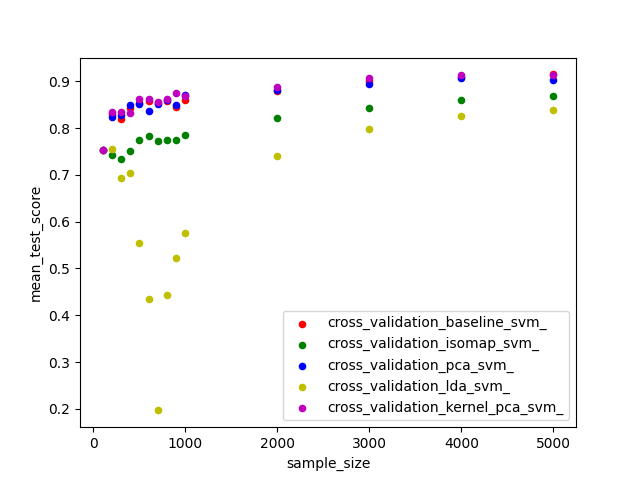
\includegraphics[width=0.8\textwidth]{figures/test_score_based_on_size.png}
    \caption{}
    \label{fig:experiment_4_performance_size}
\end{figure}


\begin{figure}[htb!]
    \centering
    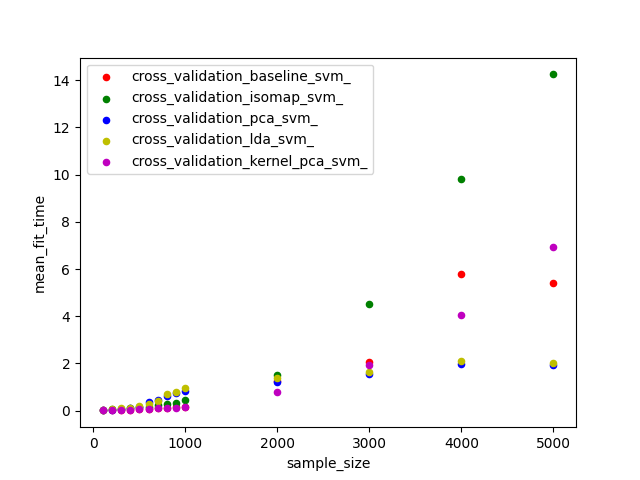
\includegraphics[width=0.8\textwidth]{figures/time_based_on_size.png}
    \caption{}
    \label{fig:experiment_4_speed_size}
\end{figure}


In terms of performance, \ref{fig:experiment_4_performance_size} shows that both baseline \gls{pca} and \gls{kpca} perform similarly well across all sample sizes, with consistently high F1 scores. In contrast, \gls{lda} performs worse overall, while \gls{isomap} has slightly lower F1 scores in smaller sample sizes but performs better in larger samples.

In terms of speed, \ref{fig:experiment_4_speed_size} shows that both \gls{pca} and \gls{lda} are the fastest when the sample size is larger than 2000, although they are slightly slower in smaller samples. Baseline \gls{pca} is the third slowest, while \gls{kpca} is the second slowest at a sample size of 5000. \gls{isomap} is the slowest overall, with longer runtimes for sample sizes of 2000 and above.

Overall, it appears that both \gls{pca} and \gls{kpca} are good choices for improving the performance of a \gls{svm} model on the \gls{mnist} data set, as they offer both high performance and fast runtime. \gls{lda} may be a less optimal choice due to its lower performance, while \gls{isomap} may be a bad option for larger sample sizes but may be suitable for smaller samples due to its slower runtime.


% The use of kernel principal component analysis  for dimensionality reduction may not have a significant impact on the performance of a support vector machine  model when applied to the \gls(mnist) data set. This is because the \gls(mnist) data set is already a low-dimensional data set, with only 784 features. In this case, using KPCA for dimensionality reduction may not provide much additional benefit, as the original data set is already well-suited for an SVM model. However, using KPCA may still have some advantages, such as the ability to remove noise and irrelevant information from the data set, and to visualize the data in a lower-dimensional space. Overall, while the use of KPCA with the \gls(mnist) data set may not have a major impact on the performance of the SVM model, it can still provide some benefits.
\chapter{Discussion}\label{cha:discussion}
Discuss the results from chapter \ref{cha:results} and compare them to the problem statement in section \ref{sec:problem-statement}. Also, discuss the methodology and the theoretical background in chapter \ref{cha:implementation}. Finally, discuss the project as a whole and the process of the project.

What went well? What could have been done better? What would we do differently next time? Perhaps include thoughts on UN sustainability goals.
\chapter{Conclusion}\label{cha:conclusion}
\chapter{Future works}\label{sec:future-works}
With the insights gained from the project, we have determined several points of interest worth looking into in the future.

Initially, the project included plans for data augmentation in the pipeline, such as slight rotation of the images or artificial errors by whitening pixels of the numbers, making this a prime candidate for future work. These augmentations would artificially increase the size of the dataset, allowing for more splits, more model accuracy, and possibly making the data more nonlinear.

The \gls{mnist} dataset is relatively simple, so it may be interesting to explore more complex datasets and study the impact of dimensionality reduction on those. Some potential datasets already mentioned in the report are the \gls{cifar} and \gls{fashion-mnist} datasets, which may increase the potential of the nonlinear approaches. Alternatively, other data types, for example, audio, would be interesting to look at because it is very different from \gls{mnist}.

Different dimensionality reduction methods would also be interesting. Especially methods not covered in depth for this report, such as \gls{nmf}, would be exciting.

Aside from different methods, \gls{kpca} has different kernels that would be interesting to explore. Section 1 shows that the choice of the kernel has a significant impact on the final accuracy. It would be interesting to explore the different kernels available.

Lastly, having access to a more powerful computer would allow us to use the nonlinear dimensionality reductions of the report on the full \gls{mnist} dataset and measure the memory usage to more accurately compare the methods' computational requirements.

Based on the discussion in chapter \ref{cha:discussion}, the results from chapter \ref{cha:results} and the problem statement in section \ref{sec:problem-statement}, we conclude:


In this project, we aimed to explore the impact of dimensionality reduction on the performance of a \gls{ml} for image classification and recognition. We focused on comparing linear and nonlinear dimensionality reduction techniques on \gls{mnist}, using a \gls{svm} as our model of choice. Our results showed that, for sample sizes greater than 2000, linear dimensionality reduction techniques were generally faster than nonlinear methods, while achieving similar levels of accuracy. This supports our hypothesis "nonlinear dimensionality reduction methods work as well as linear methods on the \gls{mnist} dataset". However, our results also indicated that nonlinear methods were more robust, in that they could remove more components before a significant drop in accuracy occurred. Overall, our findings support our hypothesis and provide valuable insights into the relative effectiveness of different dimensionality reduction techniques for image classification tasks.

In conclusion, our project has provided valuable insights into the use of dimensionality reduction techniques in image classification and recognition tasks. We have shown that, while nonlinear methods may be more computationally expensive, they can be equally as effective as linear methods in terms of performance. Our findings have important implications for the field of computer vision and can inform future research in this area.

% This chapter contains the concluding remarks of the project. It is based on the discussion in chapter \ref{cha:discussion}, the results from chapter \ref{cha:results} and the problem statement in section \ref{sec:problem-statement}. The chapter concludes with a reflection and perspectives for future work.

%backmatter
\printglossaries
\printbibliography[heading=bibintoc]\label{bib:mybiblio}

\appendix
% \begin{table}[htb!]
%     \centering
%     \begin{tabular}{cp{0.22\textwidth}p{0.26\textwidth}p{0.26\textwidth}p{0.25\textwidth}}
%         \toprule
%         \textbf{} & \textbf{PC-1} & \textbf{PC-2} & \textbf{PC-3} & \textbf{PC-4} \\
%         \midrule
%         \textbf{CPU:} & \textbf{AMD Ryzen 5600X} & \textbf{Intel Core I5-10300H} & \textbf{AMD Ryzen 5 3600} & \textbf{Intel Core I5-4460} \\
%         \textbf{RAM:} & \textbf{32GB 3200MHz} & \textbf{16GB 2900MHz} & \textbf{16GB 3600MHz} & \textbf{8GB 1600Mhz} \\
%         \bottomrule
%     \end{tabular}
%     \caption{The specifications of the four PCs used in the experiments.}
%     \label{tab:pc-specs}
% \end{table}

\begin{table}[htb!]
    \centering
    \begin{tabular}{cp{0.3\textwidth}p{0.3\textwidth}}
        \toprule
        \textbf{} & \textbf{PC-1} \\
        \midrule
        \textbf{CPU:} & \textbf{AMD Ryzen 5600X} \\
        \textbf{RAM:} & \textbf{32GB 3200MHz} \\
        \bottomrule
    \end{tabular}
    \caption{The specifications of one of the PCs used in the experiments.}
    \label{tab:pc1-specs}
\end{table}

\begin{table}[htb!]
    \centering
    \begin{tabular}{cp{0.3\textwidth}p{0.3\textwidth}}
        \toprule
        \textbf{} & \textbf{PC-2} \\
        \midrule
        \textbf{CPU:} & \textbf{Intel Core I5-10300H} \\
        \textbf{RAM:} & \textbf{16GB 2900MHz} \\
        \bottomrule
    \end{tabular}
    \caption{The specifications of one of the PCs used in the experiments.}
    \label{tab:pc2-specs}
\end{table}

\begin{table}[htb!]
    \centering
    \begin{tabular}{cp{0.3\textwidth}p{0.3\textwidth}}
        \toprule
        \textbf{} & \textbf{PC-3} \\
        \midrule
        \textbf{CPU:} & \textbf{AMD Ryzen 5 3600} \\
        \textbf{RAM:} & \textbf{16GB 3600MHz} \\
        \bottomrule
    \end{tabular}
    \caption{The specifications of one of the PCs used in the experiments.}
    \label{tab:pc3-specs}
\end{table}

\begin{table}[htb!]
    \centering
    \begin{tabular}{cp{0.3\textwidth}p{0.3\textwidth}}
        \toprule
        \textbf{} & \textbf{PC-4} \\
        \midrule
        \textbf{CPU:} & \textbf{Intel Core I5-4460} \\
        \textbf{RAM:} & \textbf{8GB 1600Mhz} \\
        \bottomrule
    \end{tabular}
    \caption{The specifications of one of the PCs used in the experiments.}
    \label{tab:pc4-specs}
\end{table}

\end{document}